%\ifdefined\isfinal\documentclass[final]{dune}\else\documentclass{dune}\fi
%\pdfoutput=1            % must be in first 5 lines so arXiv finds it
%\graphicspath{ {graphics/} {executive-summary/graphics/}{generated/} }
%% * <aheavey@fnal.gov> 2018-04-06T17:26:26.700Z:
%%
% ^.
%% stuff before document begins.  

% Most packages are required through dune.cls.  Put hyper-ref related here to assure it's last.
%%% xr won't play nice
% \usepackage{xr-hyper}
\usepackage[pdftex,bookmarks,hidelinks]{hyperref}

\graphicspath{ {graphics/} }

% make some "if"s for DP and SP.
% They should be set true inside DP or SP volume or chapter mains.
% set try like \dptrue or \sptrue.
% they can be referenced with \ifdp or \ifsp and terminated with \fi.
\newif\ifdp
\newif\ifsp




% This holds definitions of macros to enforce consistency in names.

% This file is the sole location for such definitions.  Check here to
% learn what there is and add new ones only here.  

% also see units.tex for units.  Units can be used here.

%%% Common terms

% Check here first, don't reinvent existing ones, add any novel ones.
% Use \xspace.

%%%%% Anne adding macros for referencing TDR volumes and annexes Apr 20, 2015 %%%%%
\def\expshort{DUNE\xspace}
\def\explong{The Deep Underground Neutrino Experiment\xspace}

%\def\thedocsubtitle{LBNF/DUNE Technical Design Report (DRAFT)}
\def\thedocsubtitle{Deep Underground Neutrino Experiment (DUNE)} 
%\def\tdrtitle{Technical Proposal}
\def\tdrtitle{DRAFT Technical Design Report}


% All volume titles and numbers in one place.
\def\voltitleexec{Executive Summary\xspace}
\def\volnumberexec{1}

\def\voltitlephysics{DUNE Physics\xspace}
\def\volnumberphysics{2}

\def\voltitlesp{Single-Phase Far Detector Module\xspace}
\def\volnumbersp{3}

\def\voltitledp{Dual-Phase Far Detector Module\xspace}
\def\volnumberdp{4}

\def\voltitletc{Technical Coordination\xspace}
\def\volnumbertc{5}

\def\voltitlend{Near Detector\xspace}
\def\volnumbernd{6}

\def\voltitleswc{Software and Computing\xspace}
\def\volnumberswc{7}

% see~\refsec{exec}{2.3}
\newcommand{\refsec}[2]{Volume~\csname volnumber#1\endcsname \xspace Section~#2}
% see~\refch{exec}{2}
\newcommand{\refch}[2]{Volume~\csname volnumber#1\endcsname \xspace Chapter~#2}
% see Table~\refinch{exec}{1.2}
\newcommand{\refinch}[2]{#2 in Volume~\csname volnumber#1\endcsname \xspace}

\newcommand{\bigo}[1]{\ensuremath{\mathcal{O}(#1)}}


% Things about oscillation
%
\newcommand{\numu}{\ensuremath{\nu_\mu}\xspace}
\newcommand{\nue}{\ensuremath{\nu_e}\xspace}
\newcommand{\nutau}{\ensuremath{\nu_\tau}\xspace}

\newcommand{\anumu}{\ensuremath{\bar\nu_\mu}\xspace}
\newcommand{\anue}{\ensuremath{\bar\nu_e}\xspace}
\newcommand{\anutau}{\ensuremath{\bar\nu_\tau}\xspace}

\newcommand{\dm}[1]{\ensuremath{\Delta m^2_{#1}}\xspace} % example: \dm{12}

\newcommand{\sinst}[1]{\ensuremath{\sin^2\theta_{#1}}\xspace} % example \sinst{12}
\newcommand{\sinstt}[1]{\ensuremath{\sin^22\theta_{#1}}\xspace}  % example \sinstt{12}

\newcommand{\deltacp}{\ensuremath{\delta_{\rm CP}}\xspace}   % example \deltacp
\newcommand{\mdeltacp}{\ensuremath{\delta_{\rm CP}}}   %%%%%%%%%%  <--- missing something; what's the m for?

\newcommand{\nuxtonux}[2]{\ensuremath{\nu_{#1} \to \nu_{#2}}\xspace}  % example \nuxtonux23 (no {...} )
\newcommand{\numutonumu}{\nuxtonux{\mu}{\mu}}
\newcommand{\numutonue}{\nuxtonux{\mu}{e}}
% Add chi sqd MH?  avg delta chi sqd?

% atmospheric neutrinos and PDK
\newcommand{\ptoknubar}{\ensuremath{\rightarrow K^+ \overline{\nu}}\xspace}
\newcommand{\ptoepizero}{\ensuremath{p^+ \rightarrow e^+ \pi^0}\xspace}

% Names of expts or detectors
\newcommand{\cherenkov}{Cherenkov\xspace}
\newcommand{\kamland}{KamLAND\xspace}
\newcommand{\kkande}{Kamiokande\xspace}  %%%% <---- changed to make shorter
\newcommand{\superk}{Super--Kamiokande\xspace}
\newcommand{\hyperk}{Hyper--Kamiokande\xspace}
\newcommand{\miniboone}{MiniBooNE\xspace}
\newcommand{\microboone}{MicroBooNE\xspace}
\newcommand{\minerva}{MINER$\nu$A\xspace}
\newcommand{\nova}{NO$\nu$A\xspace}
\newcommand{\numi}{NuMI\xspace}
\newcommand{\lariat}{LArIAT\xspace}
\newcommand{\argoneut}{ArgoNeuT\xspace}

% Random
\newcommand{\lartpc}{LArTPC\xspace}
\newcommand{\globes}{GLoBES\xspace}
\newcommand{\larsoft}{LArSoft\xspace}
\newcommand{\snowglobes}{SNOwGLoBES\xspace}
\newcommand{\docdb}{DUNE DocDB\xspace}
% Isotopes
\def\argon40{$^{40}$Ar}  %%%%%       <--- \Ar40 doesn't work; don't know why
\def\Ar39{$^{39}$Ar}
\def\Cl40{$^{40}$Cl}
\def\K40{$^{40}$K}
\def\B8{$^{8}$B}
\newcommand\isotope[2]{\textsuperscript{#2}#1} % use as, e.g.,: \isotope{Si}{28}

% Parameters common to SP DP
\def\fdfiducialmass{\SI{40}{\kt}\xspace}
\def\driftvelocity{\SI{1.6}{\milli\meter/\micro\second}\xspace} % same for sp and dp?
\def\lartemp{\SI{88}\,K\xspace}
\def\larmass{\SI{17.5}{\kt}\xspace} % full mass in cryostat
\def\tpcheight{\SI{12}{\meter}\xspace} % height of SP TPC, APA, CPA and of DP TPC
\def\cryostatht{\SI{14.1}{\meter}\xspace} % height of cryostat
\def\cryostatlen{\SI{62.0}{\meter}\xspace} % height of cryostat
\def\cryostatwdth{\SI{14.0}{\meter}\xspace} % height of cryostat
\def\nominalmodsize{\SI{10}{kt}\xspace} % nominal module size 10 kt

\def\dunelifetime{\SI{20}{years}\xspace} % nominal operational life time of DUNE experiment
\def\beamturnon{{2026}\xspace} % the year we expect beam to turn on
\def\firstfdmodstartinstall{{2022}\xspace} % the year we expect to start install of 1st FD moc
\def\maincavernstartexc{{2019}\xspace} % the year we expect to start cavern excavation
\def\pipiibeampower{\SI{1.2}{MW}\xspace} 


% Parameters SP
\def\spmaxfield{\SI{500}{\volt/\centi\meter}} % SPfield strength
\def\spactivelarmass{\SI{10}{\kt}\xspace} % active mass in cryostat
\def\spmaxdrift{\SI{3.52}{\m}\xspace}
\def\sptpclen{\SI{58}{\meter}\xspace} % length of SP TPC, APA, CPA
\def\apacpapitch{\SI{2.32}{\meter}\xspace} % pitch of SP CPAs and APAs
\def\spfcmodlen{\SI{3.5}{\m}} % length of SP FC module
\def\spnumch{\num{384000}\xspace} % total number of APA readout channels 
\def\spnumpdch{\num{6000}\xspace} % total number of PD readout channels 
\def\planespace{\SI{4.75}{\milli\meter}\xspace}
\def\sptargetdriftvoltpos{\SI{180}{kV}\xspace} % target drift voltage - positive

% Parameters DP
\def\dpactivelarmass{\SI{12.096}{\kt}\xspace} % active mass in cryostat
\def\dpfidlarmass{\SI{10.643}{\kt}\xspace} % fiducial mass in cryostat
\def\dpmaxdrift{\SI{12}{\m}\xspace} % max drift length
\def\dptpclen{\SI{60}{\meter}\xspace} % length of TPC
\def\dptpcwdth{\SI{12}{\meter}\xspace} % width of TPC
\def\dpswchpercrp{\num{36}\xspace} % number of anode/lem sandwiches per CRP 
\def\dpnumswch{\num{2880}\xspace} % total number of anode sandwiches in module
\def\dptotcrp{\num{80}\xspace} % total number of CRPs in module
\def\dpchpercrp{\num{1920}\xspace} %  channels per CRP
\def\dpnumcrpch{\num{153600}\xspace} % total number of CRP channels in module
\def\dpchperchimney{\num{6400}\xspace} %  channels per chimney
\def\dpnumpmtch{\num{720}\xspace} % number of PMT channels
\def\dpstrippitch{\SI{3.125}{\milli\meter}\xspace} % pitch of anode strips
\def\dpnumfcmod{\num{244}\xspace} % number of FC modules
\def\dpnumfcres{\num{240}\xspace} % number of FC resistors
\def\dpnumfcrings{\num{60}\xspace} % number of FC rings
\def\dpnominaldriftfield{\SI{500}{\volt/\cm}\xspace} % nominal drift voltage per cm
\def\dptargetdriftvoltpos{\SI{600}{\kV}\xspace} % target drift voltage - positive
\def\dptargetdriftvoltneg{\SI{-600}{\kV}\xspace} % target drift voltage - negative

% Nominal readout window time
%% SP has 2.25ms drift time.  The readout is 2*dt + 20%*dt extra.
\def\spreadout{\SI{5.4}{\ms}\xspace}
%% DP has 7.5 ms drift time.  The same (over generous) rule gives 16.5ms
\def\dpreadout{\SI{16.4}{\ms}\xspace}
% Supernova Neutrino Burst buffer and readout window time
\def\snbtime{\SI{30}{\s}\xspace}
% interesting amount of time we might have SNB neutrinos but not yet
% enough to trigger.
\def\snbpretime{\SI{10}{\s}\xspace}
% SP SNB dump size. MUST KEEP THIS MANUALLY IN SYNC 1.5 TB/s * \snbtime
\def\spsnbsize{\SI{45}{\TB}\xspace}

% keep these three numerically in sync
\def\offsitepbpy{\SI{30}{\PB/\year}\xspace}
\def\offsitegbyteps{\SI{1}{\GB/\s}\xspace}
\def\offsitegbps{\SI{8}{\Gbps}\xspace}

\def\surffnalbw{\SI{100}{\Gbps}\xspace}
\newcommand{\fnal}{Fermilab\xspace}
\newcommand{\surf}{SURF\xspace}
\newcommand{\bnl}{BNL\xspace}
\newcommand{\anl}{ANL\xspace}

% New from Anne March/April 2018
%physics terms
\newcommand{\efield}{E field\xspace}
\newcommand{\lbl}{long-baseline\xspace}
\newcommand{\Lbl}{Long-baseline\xspace}
\newcommand{\rms}{RMS\xspace} % Might want this small caps?
\newcommand{\threed}{3D\xspace}
\newcommand{\twod}{2D\xspace}

%detectors and modules
\newcommand{\fardet}{Far Detector\xspace}
\newcommand{\detmodule}{detector module\xspace}
\newcommand{\dual}{DP\xspace}
\newcommand{\Dual}{DP\xspace}
\newcommand{\single}{SP\xspace}
\newcommand{\Single}{SP\xspace}
\newcommand{\dpmod}{DP detector module\xspace}
\newcommand{\spmod}{SP detector module\xspace}
\newcommand{\lar}{LAr\xspace}
\newcommand{\lntwo}{LN$_2$\xspace}

% Top-level requirements and specifications
% 1 Minimum drift field
\def\mindriftfield{\SI{250}{\volt/\cm}\xspace}
\def\mindriftfieldgoal{\SI{500}{\volt/\cm}\xspace}
% 2 FE elec noise
\def\elecnoisefe{ \num{1000} enc\xspace}
% 3 light yield
\def\lightyield{\SI{0.5}{pe/\MeV}\xspace}
\def\lightyieldgoal{\SI{5}{pe/\MeV}\xspace}
% 4 time resolution
\def\timeres{\SI{1}{\micro/\second}\xspace}
\def\timeresgoal{\SI{100}{ns}\xspace}
% 5 LAr purity
\def\larpurity{\SI{100}{ppt}\xspace}
\def\larpuritygoal{\SI{30}{ppt}\xspace}
% 6 APA gaps
\def\apagapsame{\SI{15}{\milli\m}\xspace}
\def\apagapdiff{\SI{30}{\milli\m}\xspace}
% 7 drift field uniformity (from component positioning)
\def\fielduniformity{\SI{1}{\%}\xspace}
% 8a APA collection wire angle
\def\apacollwireangle{$\SI{0}{^\circ}$\xspace}
% 8b APA induction wire angle
\def\apainducwireangle{$\pm\SI{35.7}{^\circ}$\xspace}
% 9a APA wire pitch - U,V
\def\uvpitch{\SI{4.669}{\milli\meter}\xspace}
% 9b APA wire pitch - X, G
\def\xgpitch{\SI{4.790}{\milli\meter}\xspace}
% 10 APA wire position tolerance
\def\wirepitchtol{$\pm$\SI{0.5}{\milli\meter}\xspace}
% 11 drift field uniformity (from HVS)
\def\fielduniformityhv{\SI{1}{\%}\xspace}
% 12 HV PS ripple contrib to noise
\def\hvripplenoise{\SI{100}{enc}\xspace}
% 13 FE peaking time
\def\fepeaktime{\SI{1}{\micro\second}\xspace}
% 14 signal saturation level (SP)
\def\spsignalsat{\num{500000} electrons\xspace}
% 15 LAr N contamination
\def\nitrogencontam{\SI{25}{ppm}\xspace}
% 16 detector dead time
\def\deadtime{\SI{0.5}{\%}\xspace}
% Engineering
% 17 Cathode resistivity
\def\cathodemegohm{\SI{1}{\mega\ohm/square}\xspace}
\def\cathodegigohm{\SI{1}{\giga\ohm/square}\xspace}
% 
%\def\{\xspace}
% 19 ADC sampling frequency
\def\samplingfreq{\SI{2}{\mega\hertz}\xspace}
% 20 ADC dynamic range
\def\adcdynrange{\num{12} bits}  %{3000}:\num{1}\xspace}
\def\adcdynrangegoal{\num{13} bits} %{4070}:\num{1}\xspace}
% 21 CE power consumption (SP)
\def\cepower{\SI{50}{mW/channel}\xspace}
% 22 data to tape
\def\dataratetotape{\SI{30}{PB/year}\xspace}
% 23 SNB trigger
\def\snbtriggereff{90\% efficiency\xspace}
%\def\snbtriggervisenergy{90\% efficiency \xspace}
% 24 local E fields
\def\localefield{\SI{30}{\kV/\cm}\xspace}
% 25 non-FE noise contributions
\def\elecnoisenonfe{$\ll$ \SI{1000}{enc}\xspace}
% 26 impurity contrib from components
\def\larpuritycomps{$\ll$ \SI{30}{ppt}\xspace}
% 28 dead channels
\def\deadchannels{\SI{1}{\%}\xspace}


%detector components SP and DP
\newcommand{\dss}{DSS\xspace}
\newcommand{\hv}{high voltage\xspace}
\newcommand{\fcage}{field cage\xspace}
\newcommand{\fc}{FC\xspace}
\newcommand{\fdth}{feedthrough\xspace}
\newcommand{\fcmod}{FC module\xspace}  %%%   don't need?
\newcommand{\topfc}{top FC\xspace}
\newcommand{\botfc}{bottom FC\xspace}
\newcommand{\ewfc}{endwall FC\xspace}
\newcommand{\pdsys}{PD system\xspace}
\newcommand{\phdet}{photon detector\xspace}
\newcommand{\sipm}{SiPM\xspace}
\newcommand{\pmt}{PMT\xspace}
\newcommand{\phel}{photoelectron\xspace}
\newcommand{\pwrsupp}{power supply\xspace}
\newcommand{\pwrsupps}{power supplies\xspace}
\newcommand{\frfour}{FR-4\xspace}

% For interface tables in TDR:  (Brett put in dune.cls instead)
%\newcommand{\citedocdb}[2]{
%\href{http://docs.dunescience.org/cgi-bin/ShowDocument?docid=#1\&version=#2}{DocDB {#1}} \cite{bib:docdb#1}\xspace}  % example of use: \citedocdb{6745}{1}

% The following from phys ch-bsm 1/3/19 (was in their cls file)
\newcommand{\lsim}{{\;\raise0.3ex\hbox{$<$\kern-0.75em\raise-1.1ex\hbox{$\sim$}}\;}}
\newcommand{\gsim}{{\;\raise0.3ex\hbox{$>$\kern-0.75em\raise-1.1ex\hbox{$\sim$}}\;}}
\newcommand{\beq}{\begin{equation}}
\newcommand{\eeq}{\end{equation}}
\newcommand{\bea}{\begin{eqnarray}}
\newcommand{\eea}{\end{eqnarray}}
\newcommand{\DF}{\Delta_{4}}
\mathchardef\minus="002D
\newcommand{\dk}[1]{\textcolor{red}{#1}}
\newcommand{\dkc}[1]{\textbf{\textcolor{red}{(#1 --DK)}}}
\newcommand{\dd}[1]{\textcolor{blue}{#1}}

% This holds definitions of macros to enforce consistency in units.

% This file is the sole location for such definitions.  Check here to
% learn what there is and add new ones only here.  

% also see defs.tex for names.


% see
%  http://ctan.org/pkg/siunitx
%  http://mirrors.ctan.org/macros/latex/contrib/siunitx/siunitx.pdf

% Examples:
%  % angles
%  \ang{1.5} off-axis
%
%  % just a unit
%  \si{\kilo\tonne}
%
%  % with a value:
%  \SI{10}{\mega\electronvolt}

%  range of values:
% \SIrange{60}{120}{\GeV}

% some shorthand notation
%\DeclareSIUnit \MBq {\mega\Bq}
\DeclareSIUnit \s {\second}
\DeclareSIUnit \MB {\mega\byte}
\DeclareSIUnit \GB {\giga\byte}
\DeclareSIUnit \TB {\tera\byte}
\DeclareSIUnit \PB {\peta\byte}
\DeclareSIUnit \Mbps {\mega\bit/\s}
\DeclareSIUnit \Gbps {\giga\bit/\s}
\DeclareSIUnit \Tbps {\tera\bit/\s}
\DeclareSIUnit \Pbps {\peta\bit/\s}
\DeclareSIUnit \kton {\kilo\tonne} % changed  back to kton
\DeclareSIUnit \kt {\kilo\tonne}
\DeclareSIUnit \Mt {\mega\tonne}
\DeclareSIUnit \eV {\electronvolt}
\DeclareSIUnit \keV {\kilo\electronvolt}
\DeclareSIUnit \MeV {\mega\electronvolt}
\DeclareSIUnit \GeV {\giga\electronvolt}
\DeclareSIUnit \m {\meter}
\DeclareSIUnit \cm {\centi\meter}
\DeclareSIUnit \in {\inchcommand}
\DeclareSIUnit \km {\kilo\meter}
\DeclareSIUnit \kV {\kilo\volt}
\DeclareSIUnit \kW {\kilo\watt}
\DeclareSIUnit \MW {\mega\watt}
\DeclareSIUnit \MHz {\mega\hertz}
\DeclareSIUnit \mrad {\milli\radian}
\DeclareSIUnit \year {year}
\DeclareSIUnit \POT {POT}
\DeclareSIUnit \sig {$\sigma$}
\DeclareSIUnit\parsec{pc}
\DeclareSIUnit\lightyear{ly}
\DeclareSIUnit\foot{ft}
\DeclareSIUnit\ft{ft}
\DeclareSIUnit \ppb{ppb}
\DeclareSIUnit \ppt{ppt}
\DeclareSIUnit \samples{S}

% for a bare kt-year
\def\ktyr{\si[inter-unit-product=\ensuremath{{}\cdot{}}]{\kt\year}\xspace}
\def\Mtyr{\si[inter-unit-product=\ensuremath{{}\cdot{}}]{\Mt\year}\xspace}
\def\msr{\si[inter-unit-product=\ensuremath{{}\cdot{}}]{\meter\steradian}\xspace}
\def\ktMWyr{\si[inter-unit-product=\ensuremath{{}\cdot{}}]{\kt\MW\year}\xspace}

% used for hyphen, obsolete now: \newcommand{\SIadj}[2]{\SI[number-unit-product = -]{#1}{#2}}
% change command definition Nov 2017 in case people copy e.g., \ktadj from CDR text.
% E.g., \ktadj{10} now renders the same as \SI{10}{\kt}
\newcommand{\SIadj}[2]{\SI{#1}{#2}}

% Adjective form of some common units (Nov 2107 changed to be same as normal form, no hyphen)
% "the 10-kt detector"

\newcommand{\ktadj}[1]{\SIadj{#1}{\kt}}
% "the 1,300-km baseline"
\newcommand{\kmadj}[1]{\SIadj{#1}{\km}}
% "a 567-keV endpoint"
\newcommand{\keVadj}[1]{\SIadj{#1}{\keV}}
% "Typical 20-MeV event"
\newcommand{\MeVadj}[1]{\SIadj{#1}{\MeV}}
% "Typical 2-GeV event"
\newcommand{\GeVadj}[1]{\SIadj{#1}{\GeV}}
% "the 1.2-MW beam"
\newcommand{\MWadj}[1]{\SIadj{#1}{\MW}}
% "the 700-kW beam"
\newcommand{\kWadj}[1]{\SIadj{#1}{\kW}}
% "the 100-tonne beam"
\newcommand{\tonneadj}[1]{\SIadj{#1}{\tonne}}
% "the 4,850-foot depth beam"
\newcommand{\ftadj}[1]{\SIadj{#1}{\ft}}
%

% Mass exposure, people like to put dots between the units
% \newcommand{\ktyr}[1]{\SI[inter-unit-product=\ensuremath{{}\cdot{}}]{#1}{\kt\year}}
% must make usage of \ktyr above consistent with this one before turning on

% Beam x mass exposure, people like to put dots between the units
\newcommand{\ktmwyr}[1]{\SI[inter-unit-product=\ensuremath{{}\cdot{}}]{#1}{\kt\MW\year}}

\newcommand{\ndmuidbeamrate}{\SI[round-mode=places,round-precision=1]{20.0}{\hertz}\xspace}

\newcommand{\cosmicmuondatayear}{\SI[round-mode=places,round-precision=0]{20.4289491035}{\tera\byte}\xspace}

\newcommand{\tpcdriftdistance}{\SI[round-mode=places,round-precision=2]{3.6}{\meter}\xspace}

\newcommand{\gdaqchannelnumberfactor}{\num[round-mode=places,round-precision=1]{1.1}\xspace}

\newcommand{\daqsamplerate}{\SI[round-mode=places,round-precision=1]{2.0}{\mega\hertz}\xspace}

\newcommand{\beamspillcycle}{\SI[round-mode=places,round-precision=1]{1.2}{\second}\xspace}

\newcommand{\tpcapaperdriftcell}{\num[round-mode=places,round-precision=2]{0.75}\xspace}

\newcommand{\snbdatavolumezs}{\SI[round-mode=places,round-precision=0]{2.4e-05}{\giga\byte}\xspace}

\newcommand{\beamreprate}{\SI[round-mode=places,round-precision=2]{0.833333333333}{\hertz}\xspace}

\newcommand{\ndrockmuonrate}{\SI[round-mode=places,round-precision=1]{10.0}{\hertz}\xspace}

\newcommand{\snbdataratefs}{\SI[round-mode=places,round-precision=1]{17.5226192958}{\mega\byte\per\second}\xspace}

\newcommand{\dunefsreadoutsize}{\SI[round-mode=places,round-precision=1]{24.8832}{\giga\byte}\xspace}

\newcommand{\betarate}{\SI[round-mode=places,round-precision=1]{11.16}{\mega\hertz}\xspace}

\newcommand{\chargezsthreshold}{\SI[round-mode=places,round-precision=1]{0.5}{\MeV}\xspace}

\newcommand{\tpcmodulemass}{\SI[round-mode=places,round-precision=0]{10.0}{\kilo\tonne}\xspace}

\newcommand{\dunenumberchannels}{\num[round-mode=places,round-precision=0]{1536000.0}\xspace}

\newcommand{\chargemaxsignalnoiseratio}{\num[round-mode=places,round-precision=0]{74.0}\xspace}

\newcommand{\ndecalmass}{\SI[round-mode=places,round-precision=0]{93.0}{\tonne}\xspace}

\newcommand{\cosmicmuondatarate}{\SI[round-mode=places,round-precision=1]{647.36816}{\kilo\byte\per\second}\xspace}

\newcommand{\dunenumberapas}{\num[round-mode=places,round-precision=0]{600.0}\xspace}

\newcommand{\dunefsreadoutrate}{\SI[round-mode=places,round-precision=1]{4.608}{\tera\byte/\second}\xspace}

\newcommand{\ndecalbeamrate}{\SI[round-mode=places,round-precision=1]{18.6}{\hertz}\xspace}

\newcommand{\cosmicmuoneventsize}{\SI[round-mode=places,round-precision=1]{2.5}{\mega\byte}\xspace}

\newcommand{\tpcapapermodule}{\num[round-mode=places,round-precision=0]{150.0}\xspace}

\newcommand{\nddatarate}{\SI[round-mode=places,round-precision=1]{1.0048}{\mega\byte\per\second}\xspace}

\newcommand{\chargehethreshold}{\SI[round-mode=places,round-precision=1]{10.0}{\MeV}\xspace}

\newcommand{\beamhighdatayear}{\SI[round-mode=places,round-precision=0]{21.9254891928}{\giga\byte}\xspace}

\newcommand{\betaratedensity}{\SI[round-mode=places,round-precision=3]{0.279}{\hertz\per\kilo\gram}\xspace}

\newcommand{\cosmicmuoncorrection}{\num[round-mode=places,round-precision=2]{1.36}\xspace}

\newcommand{\snbeventratetpc}{\SI[round-mode=places,round-precision=0]{100.0}{\hertz}\xspace}

\newcommand{\snbcloserfactor}{\num[round-mode=places,round-precision=0]{100.0}\xspace}

\newcommand{\snbeventsize}{\num[round-mode=places,round-precision=0]{48.0}\xspace}

\newcommand{\beamrunfraction}{\num[round-mode=places,round-precision=3]{0.667}\xspace}

\newcommand{\beamdatayearfs}{\SI[round-mode=places,round-precision=0]{218.230533073}{\tera\byte}\xspace}

\newcommand{\tpcfulllength}{\SI[round-mode=places,round-precision=1]{58.0}{\meter}\xspace}

\newcommand{\snbcanddatayearzs}{\SI[round-mode=places,round-precision=0]{200.88}{\giga\byte}\xspace}

\newcommand{\snbdataratehighzs}{\SI[round-mode=places,round-precision=0]{2.4e-05}{\tera\byte/\second}\xspace}

\newcommand{\ndeventrate}{\SI[round-mode=places,round-precision=1]{50.24}{\hertz}\xspace}

\newcommand{\dunefsreadoutsizeyear}{\SI[round-mode=places,round-precision=1]{145.414314891}{\exa\byte}\xspace}

\newcommand{\tpcfullwidth}{\SI[round-mode=places,round-precision=1]{14.5}{\meter}\xspace}

\newcommand{\daqchannelsperapa}{\num[round-mode=places,round-precision=0]{2560.0}\xspace}

\newcommand{\tpcapaheight}{\SI[round-mode=places,round-precision=1]{6.0}{\meter}\xspace}

\newcommand{\ndbytesperchannel}{\SI[round-mode=places,round-precision=0]{5.0}{\byte}\xspace}

\newcommand{\ndmuidmass}{\SI[round-mode=places,round-precision=0]{100.0}{\tonne}\xspace}

\newcommand{\ndmuidchannels}{\num[round-mode=places,round-precision=0]{165888.0}\xspace}

\newcommand{\gdaqtrigsamplespersnhit}{\num[round-mode=places,round-precision=0]{48.0}\xspace}

\newcommand{\beamdataratefs}{\SI[round-mode=places,round-precision=0]{6.915456}{\mega\byte\per\second}\xspace}

\newcommand{\ndbeameventratedensity}{\SI[round-mode=places,round-precision=1]{0.2}{\hertz\per\tonne}\xspace}

\newcommand{\tpcapawidth}{\SI[round-mode=places,round-precision=1]{2.3}{\meter}\xspace}

\newcommand{\cosmicmuonrate}{\SI[round-mode=places,round-precision=3]{0.258947264}{\hertz}\xspace}

\newcommand{\ndsstbeamrate}{\SI[round-mode=places,round-precision=1]{1.6}{\hertz}\xspace}

\newcommand{\tpcdrifttime}{\SI[round-mode=places,round-precision=2]{2.25}{\milli\second}\xspace}

\newcommand{\snbeventsizefs}{\SI[round-mode=places,round-precision=1]{46.08}{\tera\byte}\xspace}

\newcommand{\chargeminsignalnoiseratio}{\num[round-mode=places,round-precision=0]{15.0}\xspace}

\newcommand{\beameventsizecompressed}{\SI[round-mode=places,round-precision=1]{0.1}{\mega\byte}\xspace}

\newcommand{\ndecalchannels}{\num[round-mode=places,round-precision=0]{52224.0}\xspace}

\newcommand{\ndcosmicmuonrate}{\SI[round-mode=places,round-precision=2]{0.04}{\hertz}\xspace}

\newcommand{\ndbeameventrate}{\SI[round-mode=places,round-precision=1]{40.2}{\hertz}\xspace}

\newcommand{\gdaqronetriggeredphysicsdatarate}{\SI[round-mode=places,round-precision=0]{0.8448}{\byte\per\second}\xspace}

\newcommand{\gdaqunit}{\SI[round-mode=places,round-precision=0]{0.825}{\byte}\xspace}

\newcommand{\gdaqbetahighrateAPA}{\SI[round-mode=places,round-precision=0]{500.0}{\kilo\hertz}\xspace}

\newcommand{\dunenumbermodules}{\num[round-mode=places,round-precision=0]{4.0}\xspace}

\newcommand{\daqreadoutchannelsamples}{\num[round-mode=places,round-precision=0]{10800.0}\xspace}

\newcommand{\beameventsize}{\SI[round-mode=places,round-precision=1]{2.5}{\mega\byte}\xspace}

\newcommand{\tpcdriftvelocity}{\SI[round-mode=places,round-precision=1]{1.6}{\milli\meter\per\micro\second}\xspace}

\newcommand{\gdaqronebeamphysicsdatarate}{\SI[round-mode=places,round-precision=0]{41250.0}{\kilo\byte\per\second}\xspace}

\newcommand{\gdaqronedatarate}{\SI[round-mode=places,round-precision=0]{41.5153208448}{\mega\byte\per\second}\xspace}

\newcommand{\ndsstmass}{\SI[round-mode=places,round-precision=0]{8.0}{\tonne}\xspace}

\newcommand{\beamfsdatarate}{\SI[round-mode=places,round-precision=0]{436.461066147}{\peta\byte\per\year}\xspace}

\newcommand{\snbreadouttime}{\SI[round-mode=places,round-precision=1]{10.0}{\second}\xspace}

\newcommand{\gdaqronebetadatarate}{\SI[round-mode=places,round-precision=1]{41.25}{\mega\byte\per\second}\xspace}

\newcommand{\snbcanddataratezs}{\SI[round-mode=places,round-precision=0]{6365.63904105}{\byte\per\second}\xspace}

\newcommand{\gdaqnoncosmicoverheadfactor}{\num[round-mode=places,round-precision=1]{1.5}\xspace}

\newcommand{\gdaqronelowenergyphysicsdatarate}{\SI[round-mode=places,round-precision=0]{7.92}{\kilo\byte\per\second}\xspace}

\newcommand{\gdaqcrrateAPA}{\SI[round-mode=places,round-precision=4]{0.0004}{\hertz}\xspace}

\newcommand{\beamonfraction}{\num[round-mode=places,round-precision=0]{0.0030015}\xspace}

\newcommand{\betadatayear}{\SI[round-mode=places,round-precision=0]{52.8262940816}{\peta\byte}\xspace}

\newcommand{\betainspillyear}{\SI[round-mode=places,round-precision=0]{158.558121686}{\tera\byte}\xspace}

\newcommand{\gdaqtrigcompression}{\num[round-mode=places,round-precision=0]{2.0}\xspace}

\newcommand{\gdaqhighrateAPAs}{\num[round-mode=places,round-precision=0]{100.0}\xspace}

\newcommand{\daqdriftsperreadout}{\num[round-mode=places,round-precision=1]{2.4}\xspace}

\newcommand{\snbdatavolumehighzs}{\SI[round-mode=places,round-precision=0]{0.00024}{\tera\byte}\xspace}

\newcommand{\ndsstchannels}{\num[round-mode=places,round-precision=0]{215040.0}\xspace}

\newcommand{\gdaqroneSNphysicsdatarate}{\SI[round-mode=places,round-precision=0]{257.4}{\kilo\byte\per\second}\xspace}

\newcommand{\beamhighdatarate}{\SI[round-mode=places,round-precision=2]{0.694791666667}{\kilo\byte\per\second}\xspace}

\newcommand{\dunefsreadoutsizeminute}{\SI[round-mode=places,round-precision=1]{276.48}{\tera\byte}\xspace}

\newcommand{\daqchannelspermodule}{\num[round-mode=places,round-precision=0]{384000.0}\xspace}

\newcommand{\gdaqtrigsamplesperbetahit}{\num[round-mode=places,round-precision=0]{24.0}\xspace}

\newcommand{\snbcandrate}{\SI[round-mode=places,round-precision=0]{12.0}{\per\year}\xspace}

\newcommand{\dunedetectormass}{\SI[round-mode=places,round-precision=0]{40.0}{\kilo\tonne}\xspace}

\newcommand{\gdaqAPAchannelspercosmic}{\num[round-mode=places,round-precision=0]{2560.0}\xspace}

\newcommand{\ndeventsize}{\num[round-mode=places,round-precision=0]{4000.0}\xspace}

\newcommand{\snbdatayearfs}{\SI[round-mode=places,round-precision=0]{552.96}{\tera\byte}\xspace}

\newcommand{\dunefsreadoutsizesecond}{\SI[round-mode=places,round-precision=1]{4.608}{\tera\byte}\xspace}

\newcommand{\betainbeamyear}{\SI[round-mode=places,round-precision=0]{79.279060843}{\giga\byte}\xspace}

\newcommand{\gdaqlphighrateAPA}{\SI[round-mode=places,round-precision=0]{200.0}{\hertz}\xspace}

\newcommand{\betaeventsize}{\num[round-mode=places,round-precision=1]{100.0}\xspace}

\newcommand{\betadatarate}{\SI[round-mode=places,round-precision=1]{1.674}{\giga\byte\per\second}\xspace}

\newcommand{\betareadoutsize}{\SI[round-mode=places,round-precision=0]{150.0}{\byte}\xspace}

\newcommand{\snbcandeventsizezs}{\SI[round-mode=places,round-precision=1]{16.74}{\giga\byte}\xspace}

\newcommand{\daqreadouttime}{\SI[round-mode=places,round-precision=1]{5.4}{\milli\second}\xspace}

\newcommand{\cosmicmuonflux}{\SI[round-mode=places,round-precision=2]{5.66e-09}{\hertz\per\centi\meter\squared}\xspace}

\newcommand{\snbdataratezs}{\SI[round-mode=places,round-precision=0]{2.4e-06}{\giga\byte\per\second}\xspace}

\newcommand{\tpcfullheight}{\SI[round-mode=places,round-precision=1]{12.0}{\meter}\xspace}

\newcommand{\gdaqsnhighrateAPA}{\SI[round-mode=places,round-precision=0]{6500.0}{\hertz}\xspace}

\newcommand{\beameventoccupancy}{\num[round-mode=places,round-precision=4]{0.0005}\xspace}

\newcommand{\beamrate}{\SI[round-mode=places,round-precision=0]{8770.19567714}{\per\year}\xspace}

\newcommand{\daqbytespersample}{\SI[round-mode=places,round-precision=1]{1.5}{\byte}\xspace}

% generated file, do not edit% This file is generated, any edits may be lost.

% It defines macros which expand to corresponding
% specification values for subsystem SP-FD


\def\sphvsfielduniformity{$<\,\SI{1}{\%}$ throughout volume}
\def\spadcnumberofbits{\num{12} bits}
\def\splightyield{$>\,\SI{0.5}{pe/MeV}$}
\def\sphvpsripple{$<\,\SI{100}{enc}$}
\def\spcathoderesistivity{$>\,\SI{1}{\mega\ohm/square}$}
\def\spspsignalsaturation{\num{500000} electrons}
\def\spapagaps{$<\,\SI{15}{mm}$ between APAs on same support beam; $<\,\SI{30}{mm}$ between APAs on different support beams}
\def\spradiopurity{ALARA}
\def\spfepeaktime{\SI{1}{\micro\second}}
\def\splarpurity{$<$\,\SI{100}{ppt}}
\def\spcepowerconsumption{$<\,\SI{50}{ mW/channel} $}
\def\spcryomonitordevices{}
\def\spdataratetotape{$<\,\SI{30}{PB/year}$}
\def\spdetdeadtime{$<\,\SI{0.5}{\%}$}
\def\splocalefields{$<\,\SI{30}{kV/cm}$}
\def\sptimeresolutionpds{$<\,\SI{1}{\micro\second}$}
\def\spadcsamplingfreq{$\sim\,\SI{2}{\mega\hertz}$}
\def\spsystemnoise{$<\,\SI{1000}{enc}$}
\def\spmindriftfield{$>$\,\SI{250}{ V/cm}}
\def\splarimpuritycontrib{$<<\,\SI{30}{ppt} $}
\def\spapawirespacing{\SI{4.669}{mm} for U,V; \SI{4.790}{mm} for X,G}
\def\spsntrigger{$>\,\SI{90}{\%}$ efficiency for SNB within \SI{100}{kpc}}
\def\spapawirepostolerance{$\pm\,\SI{0.5}{mm}$}
\def\spnonfenoise{$<<\,\SI{1000}{enc} $}
\def\spdeadchannels{$<\,\SI{1}{\%}$}
\def\splarncontamination{$<\,\SI{25}{ppm}$}
\def\spmisalignmentfielduniformity{$<\,1\,$\% throughout volume}
\def\spapawireangles{\SI{0}{\degree} for collection wires, \SI{35.7}{\degree} for induction wires}

% This file is generated, any edits may be lost.

% It defines macros which expand to corresponding
% specification values for subsystem DP-FD


\def\dpadcsamplingfreq{$\sim\,\SI{2.5}{\mega\hertz}$}
\def\dpcepowerconsumption{$<\,\SI{50}{ mW/channel} $}
\def\dpcrpeffgain{\num{6}}
\def\dpcrpgaps{$<\,\SI{30}{mm}$ between adjacent CRPs}
\def\dpcrpplanarity{$\pm\,\SI{0.75}{mm}$}
\def\dpcrpstripspacing{$<\,\SI{4.7}{mm}$}
\def\dpdpadcnumberofbits{\num{12} bits}
\def\dpdpcathoderesistivity{$>\,\SI{1}{\mega\ohm/square}$}
\def\dpdpcryomonitordevices{}
\def\dpdpdataratetotape{$<\,\SI{30}{PB/year}$}
\def\dpdpdeadchannels{$<\,\SI{1}{\%}$}
\def\dpdpdetdeadtime{$<\,\SI{0.5}{\%}$}
\def\dpdpfepeaktime{\SI{1}{\micro\second}}
\def\dpdphvpsripple{$<\,\SI{100}e^-$}
\def\dpdphvsfielduniformity{$<\,\SI{1}{\%}$ throughout volume}
\def\dpdplarimpuritycontrib{$<<\,\SI{30}{ppt} $}
\def\dpdplarncontamination{$<\,\SI{25}{ppm}$}
\def\dpdplocalefields{$<\,\SI{30}{kV/cm}$}
\def\dpdpmindriftfield{$>$\,\SI{250}{V/cm}}
\def\dpdpmisalignfielduniformity{$<\,1\,$\% throughout volume}
\def\dpdpnonfenoise{$<<\,\SI{1000}\,e^- $}
\def\dpdpradiopurity{less than that from $^{39}$Ar}
\def\dpdpsignalsaturation{\num{7500000} $e^-$}
\def\dpdpsntrigger{$>\,\SI{90}{\%}$ efficiency for SNB within \SI{100}{kpc}}
\def\dplarpurity{$<$\,\SI{100}{ppt}}
\def\dplightyield{$>\,\SI{1}{PE/MeV}$ (min), $>\,\SI{3}{PE/MeV}$ (avg)}
\def\dpsystemnoise{$<\,\SI{2500}\,e^-$}
\def\dptimeresolutionpds{$<\,\SI{1}{\micro\second}$}

% This file is generated, any edits may be lost.

% It defines macros which expand to corresponding
% specification values for subsystem SP-APA


\def\spapaunitsize{\SI{6.0}{m} tall $\times$ \SI{2.3}{m} wide}
\def\spapabadchannels{$<$1\%, with a goal of $<$0.5\%}
\def\spapaframeplanarity{$<$\SI{5}{mm}}
\def\spapaactivearea{Maximize total active area.}
\def\spapabiasvoltage{The setup, including boards, must hold 150\% of max operating voltage.}
\def\spapawiretension{\SI{6}{N} $\pm$ \SI{1}{N}}

% This file is generated, any edits may be lost.

% It defines macros which expand to corresponding
% specification values for subsystem SP-HV


\def\sphvconnectionredundancy{Two-fold}
\def\sppowersupplystability{}

% This file is generated, any edits may be lost.

% It defines macros which expand to corresponding
% specification values for subsystem SP-PDS


\def\sppdscablemate{$<$\SI{6}{\milli\meter}}
\def\sppdsdatarate{$<$\SI{8}{Gbps}}
\def\sppdslocation{(Dave: what is required to avoid damage)}
\def\spmechdeflection{$<$\SI{5}{\milli\meter}}
\def\sppdscompatible{$>$\SI{1}{\milli\meter}}
\def\spspatiallocalization{< \SI{100}{\cm}}
\def\spapainstall{$>$\SI{1}{\milli\meter}}
\def\splyuniformity{< \num{50}\%}
\def\spedlight{<\SI{10}{\%}}
\def\splighttightness{<\SI{10}{\%}}
\def\spenvhumiditylimit{< \SI{50}{\%} RH at \SI{70}{\degree F}}
\def\spenvlightexposure{\num{0} sunlight; ALARA other sources}
\def\sppdscable{$<$\SI{6}{\milli\meter}}

% This file is generated, any edits may be lost.

% It defines macros which expand to corresponding
% specification values for subsystem DP-PDS


\def\dpdplarnitrogencontamination{$<\,\SI{3}{ppm}$}
\def\dpdplightyield{$>\,\SI{1}{PE/MeV}$ at anode, $>\,\SI{5}{PE/MeV}$ avg over  active vol}
\def\dpdptimeresolution{$<\,\SI{1}{\micro\second}$}
\def\dphitrelativetiming{$<\,\SI{100}{ns RMS}$}
\def\dphitsnr{$>\,\num{5}$}
\def\dppdsanalogrange{$>\,\SI{100}{PE/(channel\times 6\nano\second)}$}
\def\dppmtdarkrate{$<\,\SI{100}{kHz}$}

% This file is generated, any edits may be lost.

% It defines macros which expand to corresponding
% specification values for subsystem SP-DAQ


\def\spdatarecord{}
\def\spdeadtime{}
\def\sptriggerhighenergy{$>$\SI{100}{\MeV}}
\def\sptriggercalibration{}
\def\sptriggerbeam{$>$\SI{100}{\MeV}}
\def\sptriggerlowenergy{$>$\SI{10}{\MeV}}
\def\sptriggersnb{}

% This file is generated, any edits may be lost.

% It defines macros which expand to corresponding
% specification values for subsystem SP-CISC


\def\speleclifetimeprec{$<\,$1.4\% ($<$4\%)}
\def\spinstnoise{$\ll\,\SI{1000}{enc}$}
\def\spslowcontrolarchiverate{\SI{0.02}{Hz}}
\def\sptemprepro{$<\,\SI{5}{mK}$}
\def\spslowcontrolnumvars{$>\,\num{150000}$}
\def\spcameracoldcoverage{$>\,$80\% of HV surfaces}
\def\spslowcontrolalarmrate{$<\,$150/day}
\def\sptempstability{$<\,\SI{2}{mK}$ at all places and times}
\def\speleclifetimerange{\SIrange{0}{10}{ms} (\SIrange{0}{30}{ms})}
\def\spinstefield{$<\,\SI{30}{kV/cm}$}

% This file is generated, any edits may be lost.

% It defines macros which expand to corresponding
% specification values for subsystem DP-CISC


\def\dpcameracoldcoverage{$>\,$80\% of HV surfaces}
\def\dpeleclifetimeprec{$<\,$1.4\%}
\def\dpeleclifetimerange{\SIrange{0}{10}{ms} (\SIrange{0}{30}{ms})}
\def\dpinstefield{$<\,\SI{30}{kV/cm}$}
\def\dpinstnoise{$\ll\,\SI{1000}{enc}$}
\def\dpslowcontrolalarmrate{$<\,$150/day}
\def\dpslowcontrolarchiverate{\SI{0.02}{Hz}}
\def\dpslowcontrolnumvars{$>\,\num{150000}$}
\def\dptemprepro{$<\,\SI{5}{mK}$}
\def\dptempstability{$<\,\SI{2}{mK}$ at all places and times}

% This file is generated, any edits may be lost.

% It defines macros which expand to corresponding
% specification values for subsystem SP-ELEC


\def\spcoldcablesxsec{\SI{2.5}{in}}
\def\spFEMBdatalink{\num{4} at \SI{1.28}{Gbps}}
\def\spgainFEamplifier{\sim\SI{20}{mV/fC} }
\def\spnumchannelsFEMB{}
\def\spnumFEbaselines{\num{2}}
\def\spnumberFEMBperWIB{\num{4}}
\def\spsyncronizationCE{\SI{50}{ns}}
\def\spWIBdatalink{\SI{10}{Gbps}}

% This file is generated, any edits may be lost.

% It defines macros which expand to corresponding
% specification values for subsystem SP-CALIB


\def\spdatavolumelaser{$>\,\SI{84}{TB/yr/10 kt}$}
\def\spdatavolumepns{$>\,\SI{84}{TB/yr/10 kt}$}
\def\spefieldcalibcoverage{$>\,\SI{75}{\%}$}
\def\spefieldcalibgranularity{$<\,\SI{30\times30\times30}{\centi\meter}$}
\def\spefieldcalibprecision{\SI{1}{\%}}
\def\splaserpositionprecision{\SI{0.5}{\milli\rad}}
\def\spneutronsourcecoverage{$>\,\SI{75}{\%}$}
\def\sprategammassource{$<\,\SI{1}{\kilo\hertz}$}

% This file is generated, any edits may be lost.

% It defines macros which expand to corresponding
% specification values for subsystem SP-TC


\def\spapastoragesd{na}
\def\spcleanroomspecification{na}
\def\spcleanroomuvfilters{na}
\def\splogisticsmaterialhandling{SURF Material Handling Specification}
\def\splogisticsmaterialsbuffer{$>1$ month}
\def\splogisticsshippingcoord{2 wk notice to CMGC}



% For abbrev/acronym lists, see also init.tex for entry point of acronyms.tex.
% \usepackage[intoc]{nomencl}
% \makenomenclature
% \renewcommand{\nomname}{Acronyms, Abbreviations and Terms}
% \setlength{\nomlabelwidth}{0.2\textwidth}

% For glossaries, needs to be loaded *after* hyperref to get clickable links.
% See dune-words.tex for detailed explanation.

% http://mirrors.ctan.org/macros/latex/contrib/glossaries/glossaries-user.pdf

% \usepackage[acronyms,toc]{glossaries}
\usepackage[toc]{glossaries}
\makeglossaries


% for terms with acronyms
\newcommand{\dshort}[1]{\glsentrytext{#1}}
\newcommand{\dshorts}[1]{\glsentryshortpl{#1}}
\newcommand{\dlong}[1]{\glsentrylong{#1}}
\newcommand{\dlongs}[1]{\glsentrylongpl{#1}}

% force the "first time" behavior
\newcommand{\dfirst}[1]{\glsfirst{#1}}
\newcommand{\dfirsts}[1]{\glsfirstplural{#1}}

\newcommand{\dword}[1]{\gls{#1}}
\newcommand{\dwords}[1]{\glspl{#1}}
\newcommand{\Dword}[1]{\Gls{#1}}
\newcommand{\Dwords}[1]{\Glspl{#1}}


% use this to define terms that do NOT have acronyms.
% \newduneword{label}{term}{description}
\newcommand{\newduneword}[3]{
    \newglossaryentry{#1}{
        text={#2},
        long={#2},
        name={\glsentrylong{#1}},
        first={\glsentryname{#1}},
        firstplural={\glsentrylong{#1}\glspluralsuffix},
        description={#3}
    }
}

% use this to define terms that DO have acronyms.
%                 1      2     3       4 
% \newduneabbrev{label}{abbrev}{term}{description}
\newcommand{\newduneabbrev}[4]{
  \newglossaryentry{#1}{
    text={#2},
    long={#3},
    shortplural={{#2}\glspluralsuffix},
    longplural={{#3}\glspluralsuffix{}},
    name={\glsentrylong{#1}{} (\glsentrytext{#1}{})},
    first={\glsentryname{#1}},
    firstplural={\glsentrylong{#1}\glspluralsuffix{} (\glsentrytext{#1}\glspluralsuffix{})},
    description={#4}
  }
}

%% If plural needs special spelling besides adding an "s"
%                 1      2     3       4        5
% \newduneabbrev{label}{abbrev}{term}{terms}{description}
\newcommand{\newduneabbrevs}[5]{
  \newglossaryentry{#1}{
    text={#2},
    long={#3},
    plural={#4},
    shortplural={{#2}\glspluralsuffix},
    longplural={#4},
    name={\glsentrylong{#1}{} (\glsentrytext{#1}{})},
    first={#3 (#2)},
    firstplural={#4 (\glsentrytext{#1}\glspluralsuffix{})},
    description={#5}
  }
}


% tres meta
\newduneword{dword}{DUNE Word}{A term in the DUNE lexicon}

%%%%%%     START ADDING WORDS, IN ALPHABETICAL ORDER IF POSSIBLE!    %%%%%%%%
%near detector
\newduneabbrev{nd}{ND}{near detector}{Refers to the detector(s) %or more  generally the experimental site
 installed close to the neutrino source at \fnal }

%far detector
\newduneabbrev{fd}{FD}{far detector}{Refers to the \fdfiducialmass fiducial mass DUNE detector %or more generally the experimental 
  to be installed at the far site at \surf in
  Lead, SD, to be composed of four \nominalmodsize modules}

%single-phase
\newduneabbrev{sp}{SP}{single-phase}{Distinguishes one of the DUNE far detector technologies by the fact that it operates using argon in its liquid phase only
  %Distinguishes one of the four  \SI{10}{\kton} \glspl{detmodule} of the DUNE far detector by the  fact that it operates using argon in just its liquid phase}
  }

%dual-phase
\newduneabbrev{dp}{DP}{dual-phase}{Distinguishes one of the DUNE far detector technologies by the fact that it operates using argon %Distinguishes one of the four \SI{10}{\kton} \glspl{detmodule} of the DUNE far detector by the fact that it operates using argon 
 in both gas and liquid phases}

%photon detection system
\newduneabbrev{pds}{PDS}{photon detection system}{The detector 
  subsystem sensitive to light produced in the \lar }

%time projection chamber
\newduneabbrev{tpc}{TPC}{time projection chamber}{The portion of each
  DUNE \gls{detmodule} that records ionization electrons
  after they drift away from a cathode through the \lar, and also
  through gaseous argon in a \dual module. 
  The activity is recorded by digitizing the waveforms of current
  induced on the anode as the distribution of ionization charge passes by
  or is collected on the electrode}

%anode plane assembly
\newduneabbrevs{apa}{APA}{anode plane assembly}{anode plane assemblies}{A unit of the \single
  detector module containing the elements sensitive to ionization in the \lar. 
  It contains two faces each of three planes of wires, and interfaces to the cold
  electronics and photon detection system} 

%charge readout
\newduneabbrev{cro}{CRO}{charge readout}{The system for detecting
  ionization charge distributions in a \dual detector module}

%light readout
\newduneabbrev{lro}{LRO}{light readout}{The system for detecting
  scintillation photons in a \dual  detector module}

%front-end
\newduneabbrev{fe}{FE}{front-end}{The front-end refers a point that is
  ``upstream'' of the data flow for a particular subsystem. 
  For example the front-end electronics is where the cold electronics
  meet the sense wires of the TPC and the front-end DAQ is where the
  DAQ meets the output of the electronics}

\newduneabbrev{daqrou}{RU}{DAQ readout units}{The first element in the data flow of the DAQ.}

\newduneabbrev{cots}{COTS}{commercial off-the-shelf}{Items, typically hardware such as computers, which may be purchased whole, without any custom design or fabrication and thus at normal consumer prices and availability.}


%analog digital converter
\newduneabbrev{adc}{ADC}{analog-to-digital converter}{A sampling of a voltage
  resulting in a discrete integer count corresponding in some way to
  the input}

%data acquisition
\newduneabbrev{daq}{DAQ}{data acquisition}{The data acquisition system
  accepts data from the detector FE electronics, buffers
  the data, performs a \gls{trigdecision}, builds events from the selected
  data and delivers the result to the offline \gls{diskbuffer}}

%detector module
\newduneword{detmodule}{detector module}{The entire DUNE far detector is
  segmented into four modules, each with a nominal \SI{10}{\kton}
  fiducial mass}

%detector unit
\newduneword{detunit}{detector unit}{A \gls{submodule} may be partitioned
  into a number of similar parts. 
  For example the single-phase TPC \gls{submodule} is made up of APA
  units}

%secondary DAQ buffer
\newduneword{diskbuffer}{secondary DAQ buffer}{A secondary
  \dshort{daq} buffer holds a small subset of the full rate as
  selected by a \gls{trigcommand}. 
  This buffer also marks the interface with the DUNE Offline}

%online  monitoring
\newduneabbrev{om}{OM}{online monitoring}{Processes that run inside
  the DAQ on data ``in flight,'' specifically before landing on the
  offline disk buffer, and that provide feedback on the operation of
  the DAQ itself and the general health of the data it is marshalling}

%data quality monitoring
\newduneabbrev{dqm}{DQM}{data quality monitoring}{Analysis of the raw
  data to monitor the integrity of the data and the performance of the
  detectors and their electronics. This type of monitoring may be
  performed in real time, within the \gls{daq} system, or in later
  stages of processing, using disk files as input}

%DAQ dump buffer
\newduneword{dumpbuffer}{DAQ dump buffer}{This \dshort{daq} buffer
  accepts a high-rate data stream, in aggregate, from an associated
  \gls{submodule} sufficient to collect all data likely relevant to
  a potential \gls{snb}}

%Global Trigger Logic
\newduneabbrev{etl}{ETL}{external trigger logic}{Trigger processing
  that consumes \gls{detmodule} level \gls{trignote} information
  and other global sources of trigger input and emits
  \gls{trigcommand} information back to the \glspl{mtl}}

%trigger notification
\newduneword{trignote}{trigger notification}{Information provided by
  \gls{mtl} to \gls{etl} about \gls{trigdecision} its processing}

%trigger primitive
\newduneword{trigprimitive}{trigger primitive}{Information derived by
  the DAQ \gls{fe} hardware that describes a region of space (e.g.,
  one or several neighboring channels) and time (e.g., a contiguous set
  of ADC sample ticks) associated with some activity}

%external trigger candidate
\newduneword{externtrigger}{external trigger candidate}{Information
  provided to the \gls{mtl} about events external to a
  \gls{detmodule} so that it may be considered in forming
  \glspl{trigcommand}}

%Out-of-band trigger command dispatcher
\newduneabbrev{daqoob}{OOB dispatcher}{out-of-band trigger command
  dispatcher}{This component is responsible for dispatching a \gls{snb} dump
  command to all \glspl{daqfer} in the \gls{detmodule}}

%module trigger logic
\newduneabbrev{mtl}{MTL}{module trigger logic}{Trigger processing
  that consumes \gls{detunit} level \gls{trigcommand} information
  and emits \glspl{trigcommand}. 
  It provides the \gls{etl} with \glspl{trignote} and receives back any
  \glspl{externtrigger}}

%octant
\newduneword{octant}{octant}{Any of the eight parts into which 4$\pi$
  is divided by three mutually perpendicular axes. 
  In particular in referencing the value for the mixing angle
  $\theta_{23}$}

%sub-detector ??? %%%%%%%%%%%%%%%%%%%      Why not ``subdet''? (Anne)  %%%%%% ???????
\newduneword{submodule}{subdetector}{A detector unit of granularity less
  than one \gls{detmodule} such as the TPC of either a \single or \dual 
  module}

%trigger candidate
\newduneword{trigcandidate}{trigger candidate}{Summary information derived
  from the full data stream and representing a contribution toward
  forming a \gls{trigdecision}}

%trigger command
\newduneword{trigcommand}{trigger command}{Information derived from
  one or more \glspl{trigcandidate}  that directs elements of the
  \gls{detmodule} to read out a portion of the data stream}

%trigger command message
\newduneabbrev{tcm}{TCM}{trigger command message}{A message flowing
  down the trigger hierarchy from global to local context.  Also see \gls{tpm}}

%trigger decision
\newduneword{trigdecision}{trigger decision}{The process by which
  \glspl{trigcandidate} are converted into \glspl{trigcommand}}

%trigger primitive message
\newduneabbrev{tpm}{TPM}{trigger primitive message}{A message flowing
  up the trigger hierarchy from local to global context.  Also see \gls{tcm}}

\newduneabbrev{ipc}{IPC}{inter-process communication}{A system for software elements to exchange information between threads, local processes or across a data network.  An IPC system is typically specified in terms of protocols  composed of message types and their associated data schema.}

\newduneword{daqdispre}{discovery and presence}{As used in the context of the \gls{ipc}, a system which provides mechanisms for a node on a communication network to learn of the existence of peers and their identity (discovery) as well as determine if they are currently operational or have become unresponsive (presence).}

\newduneabbrev{pubsub}{PUB/SUB}{publish-subscribe communication pattern}{An \gls{ipc} communication pattern where one element, the publisher, sends data to all connected elements, the subscribers.  Each subscriber may connect to multiple publishers.  A variant is PUB/SUB with topics where a subscriber may register an identifier, the topic, to limit the information received to just an associated subset.}

%event builder
\newduneabbrev{eb}{EB}{event builder}{A software agent servicing one
  \gls{detmodule} by executing \glspl{trigcommand} by reading out
  the requested data}

\newduneabbrev{daqdfo}{DFO}{Dataflow Orchestration}{The process by which trigger commands are executed in parallel and asynchronous manner by the back-end egress subsystem of the DAQ.}

% yes, this is a silly name
\newduneabbrev{daqfbi}{FBI}{Front-end Buffer Interfaces}{The process which provides read-only access to data residing in a front-end's buffers to processes on the network.}

%cluster on board
\newduneabbrev{cob}{COB}{Cluster On Board}{An ATCA motherboard housing four RCEs}

%reconfigurable computing element
\newduneabbrev{rce}{RCE}{reconfigurable computing element}{Data processor located outside of the cryostat on a \gls{cob} which contains \gls{fpga}, RAM and SSD resources, responsible for buffering data, producing trigger primitives, responding to triggered requests for data and sinking \gls{snb} dumps}

%bump on wire
\newduneabbrev{bow}{BOW}{Bump On Wire}{A working name for the front-end readout computing elements used in the nominal DAQ design to interface the \dual  crates to the DAQ front-end computers}

%advanced telecommunication computing architecture
\newduneabbrev{atca}{ATCA}{Advanced Telecommunications Computing
  Architecture}{An advanced computer architecture specification developed for the telecommunications, military, and aerospace industries that incorporates the latest trends high-speed interconnect technologies, next-generation processors, and improved reliability, availability and serviceability} 

%Micro Telecommunications Computing Architecture
\newduneabbrev{utca}{$\mu$TCA}{Micro Telecommunications Computing Architecture}{The computer architecture specification followed by the crates that house charge and light readout electronics in the dual-phase module} %A computer architecture. Vertical card-edge connectors, Amphenol ICC }%,  \url{https://www.amphenol-icc.com/product-series/micro-tca-card-edge.html}}

%user datagram protocol
\newduneabbrev{udp}{UDP}{user datagram protocol}{A simple,
  connectionless Internet protocol that supports data integrity
  checksums, requires no handshaking, and does not guarantee packet delivery}

%advanced meazzanine card
\newduneabbrev{amc}{AMC}{advanced mezzanine card}{Holds digitizing
  electronics and lives in \gls{utca} crates}

%radio frequency
\newduneabbrev{rf}{RF}{radio frequency}{Electromagnetic emissions
  that are within the (radio) frequency band of sensitivity of the detector
  electronics}

%field programmable gate array
\newduneabbrev{fpga}{FPGA}{field programmable gate array}{An
integrated circuit technology that allows the hardware to be reconfigured to
execute different algorithms after its manufacture and deployment}

%Front-End Link eXchange
\newduneabbrev{felix}{FELIX}{Front-End Link eXchange}{A
  high-throughput interface between front-end and trigger electronics
  and the standard PCIe computer bus}

%DAQ partition
\newduneword{daqpart}{DAQ partition}{A cohesive and
 coherent collection of DAQ hardware and software working together to trigger and read out some portion of one detector module; it consists of an integral number of \glspl{daqfrag}. 
 Multiple DAQ partitions may operate simultaneously, but each instance operates independently}

%front-end computer
\newduneabbrev{fec}{FEC}{front-end computer}{The portion of one
  \gls{daqpart} that hosts the \gls{daqdr}, \gls{daqbuf} and
  \gls{daqds}.  It is connected to the \gls{daqfer} via fiber optic. 
Each \gls{detunit} of a  certain granularity, such as two \single \glspl{apa}, has one front-end computer
  that receives data from the readout hardware, hosts the primary DAQ
  memory buffer for that data, emits trigger candidates derived from
  that data, and satisfies requests for producing subsets of that data
  for egress}

%DAQ front-end fragment
\newduneword{daqfrag}{DAQ front-end fragment}{The portion of one
  \gls{daqpart} relating to a single \gls{fec} and corresponding to an
  integral number of \glspl{detunit}.  See also \gls{datafrag}}

%data fragment
\newduneword{datafrag}{data fragment}{A block of data read out from a single \gls{daqfrag} that
span a contiguous period of time as requested by a \gls{trigcommand}}

%DAQ front-end redout
\newduneabbrev{daqfer}{FER}{DAQ front-end readout}{The portion of a
  \gls{daqfrag} that accepts data from the detector electronics and
  provides it to the \gls{fec}. 
  In the nominal design it is also responsible for generating channel
  level \glspl{trigprimitive}}

%DAQ data receiver
\newduneabbrev{daqdr}{DDR}{DAQ data receiver}{The portion of the
  \gls{daqfrag} that accepts data from the \gls{daqfer}, emits
  trigger candidates produced from the input trigger primitives, and
  forwards the full data stream to the \gls{daqbuf}}

%primary DAQ buffer
\newduneabbrev{daqbuf}{primary buffer}{DAQ primary buffer}{The portion
  of the \gls{daqfrag} that accepts full data stream from the
  corresponding \gls{detunit} and retains it sufficiently long for it
  to be available to produce a \gls{datafrag}}

%data selector
\newduneword{daqds}{data selector}{The portion of the \gls{daqfrag}
  that accepts \glspl{trigcommand} and returns the corresponding
  \gls{datafrag}.  Not to be confused with \gls{daqdsn}.}
\newduneword{daqdsn}{data selection}{The process of forming a trigger decision for selecting a subset of detector data for output by the DAQ from the content of the detector data itself.  Not to be confused with \gls{daqds}.}

%front-end mother board
\newduneabbrev{femb}{FEMB}{front-end mother board}{Refers a unit of
  the \gls{sp} cold electronics that contains the front-end amplifier
  and ADC ASICs covering 128 channels}

%application-specific integrated circuit
\newduneword{asic}{ASIC}{application-specific integrated circuit}

%low voltage
\newduneword{lv}{LV}{low voltage}

%coldata
\newduneword{coldata}{COLDATA}{a 64-channel control and communications ASIC}
%\newduneabbrev{coldata}{COLDATA}{a 64-channel control and communications ASIC}{A key component of the 128-channel \gls{femb} that provides a control and communication interface between cold \gls{lvds} channels and warm electronics external to the cryostat}

%liquid argon application-specific integrated circuit
\newduneword{larasic}{LArASIC}{A 16-channel front-end ASIC that provides signal amplification and pulse shaping}

%complementary metal-oxide-semiconductor
\newduneword{cmos}{CMOS}{Complementary metal-oxide-semiconductor}

%equivalent noise charge
\newduneword{enc}{ENC}{equivalent noise charge}

%dynamic range enhancement
\newduneword{dre}{DRE}{dynamic range enhancement}

%successive approximation register
\newduneword{sar}{SAR}{successive approximation register}

%protodune
\newduneword{protodune}{ProtoDUNE}{Either of the two DUNE prototype detectors constructed at CERN and operated in
  a CERN test beam (expected fall 2018). 
  One prototype implements \single and the other \dual technology}

%the single-phase ProtoDUNE detector
\newduneword{pdsp}{ProtoDUNE-SP}{The \single ProtoDUNE detector}

%the dual-phase ProtoDune detector
\newduneword{pddp}{ProtoDUNE-DP}{The \dual ProtoDUNE detector}

%WA105 dual-phase demonstrator
\newduneword{wa105}{WA105 DP demonstrator}{The \SI[product-units=power]{3x1x1}{m} WA105 dual-phase prototype detector at CERN}

%data aquisition event block --- includes dirty word: "event"
\newduneword{rawevent}{DAQ event block}{The unit of data output by the
  DAQ. 
  It contains trigger and detector data spanning a unique, contiguous
  time period and a subset of the detector channels.}

%solid-state disk
\newduneabbrev{ssd}{SSD}{solid-state disk}{Any storage device that
  may provide sufficient write throughput to receive, both collectively and
  distributed, the sustained full rate of data from a \gls{detmodule}
  for many seconds}

%high-level trigger --- fixme: this needs improvement
\newduneabbrev{hlt}{HLT}{high-level trigger}{A source of triggering at
  the module level}

%particle identification
\newduneabbrev{pid}{PID}{particle ID}{Particle identification}

%readout window
\newduneword{readout window}{readout window}{A fixed, atomic and
  continuous period of time over which data from a \gls{detmodule}, in
  whole or in part, is recorded. 
  This period may differ based on the trigger that initiated the
  readout}

%zero-suppression
\newduneabbrev{zs}{ZS}{zero-suppression}{Used to delete some portion of a
  data stream that does not significantly deviate from zero or
  intrinsic noise levels. 
  It may be applied at different granularity from per-channel to per
  \dword{detunit}}

%run control ------- fixme: maybe another sentence
\newduneabbrev{rc}{RC}{run control}{The system for configuring,
  starting and terminating the DAQ}

\newduneabbrev{ccm}{CCM}{control, configuration and monitoring}{A system for controlling, configuring and monitoring other systems in particular those that make up the DAQ where the CCM encompasses \gls{rc}.}

\newduneword{daqrun}{DAQ run}{A period of time over which relevant data taking conditions and DAQ configuration are asserted to be unchanged. 
  Multiple DAQ runs may occur simultaneously when multiple \glspl{daqpart} are active. 
  This term should not be confused with DUNE experiment or beam ``runs'' which typically span many DAQ runs.}
\newduneword{daqrunnum}{DAQ run number}{A monotonic increasing count which uniquely and globally identifies a \gls{daqrun}.}

%supernova neutrino burst  
\newduneabbrev{snb}{SNB}{supernova neutrino burst}{A prompt 
  increase in the flux of low-energy neutrinos emitted in the first few seconds of a core-collapse supernova.  It can also refer to a trigger command type that may be due to an SNB,
  or detector conditions that mimic its interaction signature}

%supernova burst and low energy
\newduneabbrev{snble}{SNB/LE}{supernova neutrino burst and low
  energy}{Supernova neutrino burst and low-energy physics program}

%supernova early warning system
\newduneabbrev{snews}{SNEWS}{SuperNova Early Warning System}{A global
  supernova neutrino burst trigger formed by a coincidence of SNB
  triggers collected from participating experiments}

%one pulse per second signal
\newduneabbrev{pps}{1PPS signal}{one-pulse-per-second signal}{An
  electrical signal with a fast rise time and that arrives in real
  time with a precise period of one second}

%spill location system
\newduneabbrev{sls}{SLS}{spill location system}{A system residing at
  the DUNE far detector site that provides information, possibly
  predictive, indicating periods of time when neutrinos are being
  produced by the \fnal Main Injector beam spills}

%warm interface board
\newduneabbrev{wib}{WIB}{warm interface board}{Digital electronics
  situated just outside the \single cryostat that receives digital data
  from the FEMBs over cold copper connections and sends it to the RCE
  FE readout hardware}

%network interfce controller
\newduneabbrev{nic}{NIC}{network interface controller}{Hardware for controlling the interface to a communication network.  Typically, one that obeys the Ethernet protocol}

%warm interface electronics crate
\newduneabbrev{wiec}{WIEC}{warm interface electronics crate}{Crates mounted on the signal flanges that contain the warm interface boards}

%power and timing cards
\newduneabbrev{ptc}{PTC}{power and timing cards}{Cards that provide further processing and distribution of the signals entering and exiting the \single cryostat}

%silicon photomultipler
\newduneabbrev{sipm}{SiPM}{silicon photomultiplier}{A solid-state
  avalanche photodiode sensitive to single \phel signals}

%cryogenic instrumentation and slow control
\newduneabbrev{cisc}{CISC}{cryogenic instrumentation and slow controls}{A DUNE
  consortium responsible for the cryogenic instrumentation and slow controls components}

%consortium
\newduneword{consortium}{consortium}{A unit of organization in the
  DUNE project focused on one major component of the far detector}

%art 
\newduneword{art}{\textit{art}}{A software framework implementing an
  event-based execution paradigm} %http://art.fnal.gov/

%sequential access via metadata  
\newduneabbrev{sam}{SAM}{sequential
  access via metadata}{A data-handling system to store and retrieve
  files and associated metadata, including a complete record of the
  processing that has used the files}

%art data aquisition
\newduneword{artdaq}{\textit{art}DAQ}{A general-purpose \fnal data acquisition framework for distributed data combination and processing. 
It is designed to exploit the parallelism that is possible with
modern multi-core and networked computers}

%big-O notation
\newduneword{order}{$\mathcal{O}(n)$}{of order $n$}

%\newduneword{3d}{3D}{3 dimensional (also 1D, 2D, etc.)} % not phys 
%(Use defs.tex version}
%.........

%beamline
\newduneword{beamline}{beamline}{A sequence of control and monitoring devices used for the formation of a directed collection of particles}
%conceptual design report
\newduneabbrev{cdr}{CDR}{conceptual design report}{A formal project
  document %required by funding agencies
   that describes the experiment
  at a conceptual level}

%conventional facilities
\newduneabbrev{cf}{CF}{conventional facilities}{Pertaining to
  construction and operation of buildings or caverns and conventional infrastructure}

%charge parity
\newduneabbrev{cp}{CP}{charge parity}{Product of charge and parity
  transformations}

%product of charge, parity and time-reversal
\newduneword{cpt}{CPT}{product of charge, parity
  and time-reversal transformations}

%charge-parity symmetry violation
\newduneabbrev{cpv}{CPV}{charge-parity symmetry violation}{Lack of
  symmetry in a system before and after charge and parity
  transformations are applied}

%us department of energy
\newduneword{doe}{DOE}{U.S. Department of Energy}

%deep underground neutrino experiment
\newduneword{dune}{DUNE}{Deep Underground Neutrino Experiment}

%environment, safety and health
\newduneword{esh}{ES\&H}{Environment, Safety and Health}

%fine-grained tracker
\newduneabbrev{fgt}{FGT}{fine-grained tracker}{A near detector module ??}

%far site conventional facilities
\newduneabbrev{fscf}{FSCF}{far site conventional facilities}{The
  \gslpl{cf} at the DUNE far detector site, \surf}
  
%near site conventional facilities
\newduneabbrev{nscf}{NSCF}{near site conventional facilities}{The
  \gslpl{cf} at the DUNE near detector site, \fnal}

%grand unified theory
\newduneabbrev{gut}{GUT}{grand unified theory}{A class of theories that
  unifies the electro-weak and strong forces}

%liquid argon
\newduneabbrev{lar}{LAr}{liquid argon}{The liquid phase of argon}

%liquid argon time-projection chamber
\newduneabbrev{lartpc}{LArTPC}{liquid argon time-projection chamber}{A
  class of detector technology that forms the basis for the DUNE far
  detector modules. 
  It typically entails observation of ionization activity by
  electrical signals and of scintillation by optical signals}

%long-baseline
\newduneabbrev{lbl}{LBL}{long-baseline}{Refers to the distance between the 
  neutrino source  and the far detector.  It can also refer to the distance between the near and far detectors. 
  The ``long'' designation is an approximate and relative distinction. For DUNE, this distance  (between \fnal and \surf) is approximately \SI{1300}{km}}

%long-baseline neutrino facility
\newduneabbrev{lbnf}{LBNF}{Long-Baseline Neutrino Facility}{The
  organizational entity responsible for developing the neutrino beam, the cryostats
  and cryogenics systems, and the conventional facilities for DUNE}

%mass hierarchy
\newduneabbrev{mh}{MH}{mass hierarchy}{Describes the separation
  between the mass squared differences related to the solar and
  atmospheric neutrino problems}

%fnal main injector
\newduneabbrev{mi}{MI}{\fnal Main Injector}{An accelerator at
  \fnal that provides a beam of high-energy protons that upon
  striking a target produce secondaries that decay to provide the
  neutrinos directed toward the DUNE far detector}

%protons on target
\newduneabbrev{pot}{POT}{protons on target}{Typically used as a unit
  of normalization for the number of protons striking the neutrino
  production target}

%quality assurance
\newduneabbrev{qa}{QA}{quality assurance}{The process by which quality is maintained so as to preserve
high availability and precise function}

%quality control
\newduneabbrev{qc}{QC}{quality control}{A system of maintaining
  quality through testing products against a specification}

%standard model
\newduneabbrev{sm}{SM}{Standard Model}{Refers to a theory describing
  the interaction of elementary particles}

%technical design report
\newduneabbrev{tdr}{TDR}{technical design report}{A formal project
  document %required by funding agencies 
  that describes the experiment at a technical level}

%interim design report
\newduneabbrev{tp}{IDR}{interim design report}{An intermediate
milestone on the path to a full \gls{tdr}} % changed from ``technical proposal'' 6/6/2018

%%%%%%%%%%%%% PROJECT AND PHYSICS VOLUME list for acronyms below %%%%%%%%%%%%
\newduneabbrev{ckm}{CKM matrix}{Cabibbo-Kobayashi-Maskawa
  matrix}{Refers to the matrix describing the mixing between mass and
  weak eigenstates of quarks}

\newduneabbrev{cl}{CL}{confidence level}{Refers to a probability
  used to determine the value of a random variable given its
  distribution}

\newduneabbrev{pmns}{PMNS matrix}{Pontecorvo-Maki-Nakagawa-Sakata
  matrix}{Describes the mixing between mass and weak eigenstates of
  the neutrino}



%%%%%%%%%%%%%%%%%.....................

%%%%%%%%%%%%% PROJECT AND DETECTORS VOLUME list for acronyms below %%%%%%%%%%%%

% fixme: should not have degenerate definition.  This also should be an abbrev.
%\newduneword{blm}{BLM}{(in Volume 4) beamline measurement (system); (in Volume 3) beam loss monitor} (not used -- yet! Anne 10 May 2018)
%omit trailing period in newduneabbrev(s) and newduneword, glossaries package will append the end of sentence period - Ddm

\newduneabbrevs{cpa}{CPA}{cathode plane assembly}{cathode plane assemblies}{The component of the \single detector module that provides the drift HV cathode}

\newduneabbrev{fc}{FC}{field cage}{The component of a LArTPC that contains and shapes the applied \efield}

\newduneword{cpafc}{CPA/FC}{A pair of \gls{cpa} panels and the top and bottom \gls{fc} portions that attach to the pair; an intermediate assembly for installation into the \gls{spmod} }

\newduneabbrev{topfc}{top FC}{top field cage}{The horizontal portions of the \single FC on the top}

\newduneabbrev{botfc}{bottom FC}{bottom field cage}{The horizontal portions of the \single FC on the bottom}

\newduneabbrev{ewfc}{endwall FC}{endwall field cage}{The vertical portions of the \single FC near the wall}

\newduneabbrev{gp}{GP}{ground plane}{An electrode that is held to be
  electrically neutral relative to Earth ground voltage}

  \newduneword{gg}{ground grid}{An electrode that is held to be
  electrically neutral relative to Earth ground voltage  ??}


\newduneabbrev{alara}{ALARA}{as low as reasonably
  achievable}{Typically used with regard management of radiation
  exposure but may be used more generally. It means making every
  reasonable effort to maintain e.g., exposures, to as far below the
  limits as practical, consistent with the purpose for that the
  activity is undertaken}

\newduneabbrev{ecal}{ECAL}{electromagnetic calorimeter}{A detector
  component that measures energy deposition of traversing particles}

\newduneabbrev{hv}{HV}{high voltage}{Generally describes a voltage
  applied to drive the motion of free electrons through some media}

% can also use in the text: \dword{sp} \dword{detmodule} 
\newduneword{spmod}{SP module}{single-phase detector module}
\newduneword{dpmod}{DP module}{dual-phase detector module}

\newduneabbrev{tc}{TC}{technical coordination}{A dedicated DUNE
  project effort responsible for assuring proper interfaces between
  the collaboration consortia}


%%%%%%%%%%%%% PHYSICS AND DETECTORS VOLUME list for acronyms below %%%%%%%%%%%%

\newduneabbrev{cc}{CC}{charged current}{Refers to an interaction
  between elementary particles where a charged weak force carrier
  ($W^+$ or $W^-$) is exchanged}


\newduneabbrev{dis}{DIS}{deep inelastic scattering}{Refers to
  interaction of an elementary charged particle with a nucleus in an
  energy range where the interaction can be modeled as being with
  individual nucleons}

\newduneabbrev{fsi}{FSI}{final-state interactions}{Refers to
  interactions between elementary or composite particles subsequent to
  the initial, fundamental particle interaction, such as may occur as
  the products exit a nucleus}

\newduneabbrev{geant4}{Geant4}{GEometry ANd Tracking, version 4}{A
  software toolkit for the simulation of the passage of particles
  through matter using Monte Carlo methods}

\newduneabbrev{genie}{GENIE}{Generates Events for Neutrino Interaction
  Experiments}{Software providing an object-oriented neutrino
  interaction simulation resulting in kinematics of the products of
  the interaction}

\newduneabbrev{mc}{MC}{Monte Carlo}{Refers to a method of numerical
  integration that entails the statistical sampling of the integrand
  function. 
  Forms the basis for some types of detector and physics simulations}

\newduneabbrev{qe}{QE}{quasi-elastic}{Refers to interaction between
  elementary particles and a nucleus in an energy range where the
  interaction can be modeled as occurring between constituent quarks
  of one nucleon and resulting in no bulk recoil of the resulting
  nucleus}

%%%%%%%%%%%%%%%%%%%%%%%%% PROJECT VOLUME list for acronyms below %%%%%%%%%%%%%%%

\newduneabbrev{mou}{MOU}{memorandum of understanding}{A document
  summarizing an agreement between two or more parties}

\newduneabbrev{pip2}{PIP-II}{Proton Improvement Plan II}{A plan for
  improving the protons on target delivered for the DUNE neutrino
  production beam. 
  This is revision two of this plan and is planned to be followed by a PIP-III}

\newduneabbrev{sdsta}{SDSTA}{South Dakota Science and Technology
  Authority}{The legal entity that manages the Sanford Underground
  Research Facility, \surf, in Lead, S.D}

\newduneabbrev{wbs}{WBS}{work breakdown structure}{An organizational
  project management tool by which the tasks to be performed are
  partitioned in a hierarchical manner}

%%%%%%%%%%%%%%%%%%%%%%%%% PHYSICS VOLUME list for acronyms below %%%%%%%%%%%%%%%
\newduneabbrev{br}{BR}{branching ratio}{A fractional probability for a
  decay of a composite particle to occur into some specified set or
  sets of products}

\newduneabbrev{dm}{DM}{dark matter}{The term given to the unknown
  matter or force that explains measurements of motion of galaxies
  that are otherwise inconsistent with the amount of mass associated
  with observed amount of photon production}

\newduneabbrev{dsnb}{DSNB}{Diffuse Supernova Neutrino Background}{The
  term describing the pervasive, constant flux of neutrinos due to all
  past supernova neutrino bursts}

\newduneabbrev{globes}{GLoBES}{General Long-Baseline Experiment
  Simulator}{A software package for simulating energy spectra of
  neutrino flux, interaction and measured (after application of some
  model of a detector response) energy spectra}


% are these really used anywhere?
%\newduneword{l/e}{L/E}{length-to-energy ratio}
%\newduneword{lri}{LRI}{long-range interactions}
%\newduneword{solarmass}{$M_{\odot}$}{solar mass}

\newduneabbrev{nc}{NC}{neutral current}{Refers to an interaction
  between elementary particles where a neutrally charged weak force carrier
  ($Z^0$) is exchanged}

\newduneabbrev{nh}{NH}{normal hierarchy}{Refers to the neutrino mass
  eigenstate ordering whereby the sign of the mass squared difference
  associated with the atmospheric neutrino problem is positive}

\newduneabbrev{ih}{IH}{inverted hierarchy}{Refers to the neutrino mass
  eigenstate ordering whereby the sign of the mass squared difference
  associated with the atmospheric neutrino problem is negative}

\newduneabbrev{nsi}{NSI}{nonstandard interactions}{A general class of
  theory of elementary particles other than the Standard Model}

\newduneabbrev{msw}{MSW}{Mikheyev-Smirnov-Wolfenstein effect}{Explains
  the oscillatory behavior of neutrinos produced inside the sun as
  they traverse the solar matter}

% \newduneword{sme}{SME}{Standard-Model Extension}

\newduneabbrev{susy}{SUSY}{supersymmetry}{Theoretical symmetry between a fermion and a boson}

\newduneabbrev{wimp}{WIMP}{weakly-interacting massive particle}{A
  hypothesized particle that may be a component of dark matter}

%%%%%%%%%%%%%%%%%%%%%%%%% DETECTORS VOLUME list for acronyms below %%%%%%%%%%%%%%%

\newduneabbrev{ce}{CE}{cold electronics}{Refers to readout electronics that operate at cryogenic temperatures}

\newduneabbrev{crp}{CRP}{charge-readout plane}{In the \dual technology, a  collection of
  electrodes in a planar arrangement placed at a particular voltage
  relative to some applied \efield such that drifting electrons
  may be collected and their number and time may be measured}

\newduneabbrev{dram}{DRAM}{dynamic random access memory}{A computer memory technology}

% these should be abbrev and maybe combined.
\newduneword{fermilab}{\fnal}{Fermi National Accelerator Laboratory (in Batavia, IL, the Near Site)}
\newduneword{fnal}{FNAL}{see \fnal}


\newduneabbrev{fs}{FS}{full stream}{Relates to a data stream that has not undergone selection, compression or other form of reduction}

\newduneabbrev{lem}{LEM}{large electron multiplier}{A micro-pattern detector suitable for use in ultra-pure argon vapor; LEMs consist of copper-clad PCB boards with sub-millimeter-size holes through which electrons undergo amplification}
%\newduneabbrev{lem}{LEM}{large electron multiplier}{A technique of electron multiplication via avalanche in sub-millimeter-size holes in a
%millimeter-thick printed circuit board where electric fields are understood}
\newduneabbrev{lng}{LNG}{liquefied natural gas}{Pertaining to natural gas in its liquid phase}

% this is pretty generic and isn't referenced.
%\newduneword{mesh}{mesh screen}{A fine mesh screen, glued directly to
%  the steel frame on both sides of each APA in the single-phase TPC,
% creates a uniform ground layer beneath the wire planes}

\newduneabbrev{mip}{MIP}{minimum ionizing particle}{Refers to a
  momentum traversing some medium such that the particle is losing
  near the minimum amount of energy per distance traversed} % some \mip and some \dword{mip}. If time, rectify. ??

%\newduneword{abc}{MTS}{Materials Test Stand}
%\newduneword{muid}{MuID}{muon identifier (detector)}

%\newduneword{abc}{OPERA}{Oscillation Project with Emulsion-Racking Apparatus (experiment at LNGS)}
%\newduneword{abc}{NND}{(used only in Volume 4 Chapter 7) near neutrino detector, same as ND}
%\newduneword{abc}{OD}{outer diameter}

% there is also pds
\newduneabbrev{pd}{PD}{photon detector}{Refers to the detector
  elements involved in measurement of number and arrival times of
  optical photons produced in a detector module} %volume}

\newduneabbrev{pmt}{PMT}{photomultiplier tube}{A device that makes use
  of the photoelectric effect to produce an electrical signal from the
  arrival of optical photons}

\newduneabbrev{ppm}{ppm}{parts per million}{A number equal to $10^{-6}$}
\newduneabbrev{ppb}{ppb}{parts per billion}{A number equal to $10^{-9}$}
\newduneabbrev{ppt}{ppt}{parts per trillion}{A number equal to $10^{-12}$}

\newduneword{rio}{RIO}{reconfigurable input output}

\newduneword{rpc}{RPC}{resistive plate chamber}
\newduneword{s/n}{S/N}{signal-to-noise (ratio)}
\newduneword{ssp}{SSP}{SiPM signal processor}
\newduneword{sbn}{SBN}{Short-Baseline Neutrino program (at \fnal)}
\newduneword{stt}{STT}{straw tube tracker}
%\newduneword{abc}{SURF (also Sanford Lab)}{Sanford Underground Research Facility (in Lead, SD, the Far Site)}
\newduneword{tr}{TR}{transition radiation}
%\newduneword{abc}{W}{Watt (also mW, kW, MW) }
%\newduneword{abc}{WA105}{Single-Phase LArTPC and the Long Baseline Neutrino Observatory Demonstration}
\newduneword{wire board}{wire board}{At the head end of the APA in the \single TPC, stacks of electronics boards referred to as ``wire boards'' are arrayed to anchor the wires.  They also provide the connection between the wires and the cold electronics} %?? long for a word. ??

\newduneabbrev{wls}{WLS}{wavelength shifting}{A material or process by
  which incident photons are absorbed by a material and photons are
  emitted at a different, typically longer, wavelength}

\newduneabbrev{tpb}{TPB}{tetra-phenyl butadiene}{A type of wavelength shifting material}

\newduneabbrev{sft}{SFT}{signal feedthrough}{A cryostat penetration allowing for the passage of cables or other extended parts}
\newduneabbrev{sftchimney}{SFT chimney}{signal feedthrough chimney}{In the \dual technology, a volume above the cryostat penetration used for a signal feedthrough}


\newduneword{catiroc}{CATIROC}{charge and time integrated readout chip}

\newduneabbrev{wr}{WR}{White Rabbit}{A component of the timing system that forwards clock signal and time-of-day reference data to the master timing unit}

\newduneabbrev{mch}{MCH}{MicroTCA Carrier Hub}{An network switching device}

\newduneabbrev{wrmch}{WR-MCH}{White Rabbit \gls{utca} Carrier Hub}{add def} %??

\newduneword{cmp}{CMP}{configuration management plan}

\newduneword{qap}{QAP}{quality assurance plan} %{A project management device for planning \gls{qa}}

\newduneword{ieshp}{IESHP}{integrated environmental, safety and health plan}%{Refers to the LBNF/DUNE project planning instrument}

\newduneword{dmp}{DMP}{data management plan} %{A project management device to state how the experimental data will be managed}

\newduneword{qam}{QAM}{quality assurance manager} %{The manager of \gls{qa} for the LBNF/DUNE project}

\newduneabbrev{dss}{DSS}{detector support system}{The system used to support the \single detector within the cryostat}

\newduneabbrev{itf}{ITF}{integration and test facility}{A facility where various detector components will be tested prior to installation}

\newduneabbrev{tco}{TCO}{temporary construction opening}{An opening in the side of a cryostat through which detector elements are brought into the cryostat; utilized during construction and installation}

\newduneabbrev{uit}{UIT}{underground installation team}{An organizational unit responsible for installation in the underground area at the \surf site}

\newduneabbrev{pdr}{PDR}{preliminary design review}{A project management device by which an early design is reviewed}
\newduneabbrev{fdr}{FDR}{final design review}{A project management device by which a final design is reviewed}
\newduneabbrev{prr}{PRR}{production readiness review}{A project management device by which the production readiness is reviewed}
\newduneabbrev{orr}{ORR}{operational readiness review}{A project management device by which the operational readiness is reviewed}
\newduneabbrev{ppr}{PPR}{production progress review}{A project management device by which the progress of production is reviewed}
\newduneabbrev{edms}{EDMS}{electronic document management system}{A computerized system used at CERN by which documents are managed}

\newduneword{wrgm}{WR grandmaster}{White Rabbit grandmaster}


%%%%% Software and computing %%%%

\newduneword{larsoft}{\larsoft}{Liquid Argon Software (\larsoft),  a shared base of physics software across \lartpc experiments}
\newduneword{nova}{\nova}{The \nova off-axis neutrino oscillation experiment at \fnal }
\newduneword{minerva}{\minerva}{The \minerva neutrino cross sections experiment at \fnal }
\newduneword{microboone}{\microboone}{The \lartpc-based \microboone neutrino oscillation experiment at \fnal }
\newduneword{wirecell}{wire-cell}{A tomographic automated \threed neutrino event reconstruction method for \lartpc{}s}
\newduneword{ftslite}{F-FTS-lite}{Light-weight version of the \fnal File Transfer system used for rapid data transfers out of the online systems}
\newduneword{fts}{FTS}{File Transfer System developed at \fnal to catalog and move data to permanent storage}

%%% new ones that I haven't categorized (Anne)
\newduneword{35t}{35 ton prototype}{The 35 ton prototype cryostat and \gls{sp} detector built at \fnal before the \gls{protodune} detectors}

\newduneabbrev{cuc}{CUC}{central utility cavern}{The central underground cavern  containing utilities such as central cryogenics and other systems, and the underground data center and control room}
\newduneabbrev{cfd}{CFD}{computational fluid dynamics}{High performance computer-assisted modeling of fluid dynamical systems}
\newduneword{vuv}{VUV}{vacuum ultra-violet}
\newduneword{tallbo}{TallBo}{A cylindrical cryostat at \fnal primarily used for developing scintillation light collection technologies for \lartpc detectors}

\newduneabbrev{eos}{EOS}{EOS}{The XRootD based distributed file system developed by CERN}
\newduneabbrev{ehn1}{EHN1}{Experiment Hall North One}{Location at CERN of the ProtoDUNE experiments}
\newduneword{led}{LED}{Light-emitting diode}
\newduneword{rtd}{RTD}{Cryostat level and temperature monitoring devices}
\newduneword{swc}{SWC}{Software \& Computing}
\newduneabbrev{las}{LAS}{LEM-anode Sandwich}{In the \dual technology, a \gls{lem} and its corresponding anode are mounted together in a module called a LEM-anode sandwich}

\newduneword{roi}{ROI}{region of interest}
\newduneword{hpc}{HPC}{high-performance computing facilities; generally computing facilities emphasizing parallel computing with aggregate power of more than a teraflop}


\newduneword{comfund}{common fund}{The shared resources of the collaboration}
\newduneabbrev{ims}{IMS}{integrated master schedule}{A project management device consisting of linked tasks and milestones}

\newduneword{hvdb}{HVDB}{dual-phase HV divider board}
\newduneword{sas}{SAS}{A pass-through chamber used to ensure safe transfer of materials, avoiding contamination in both directions}

\newduneword{fea}{FEA}{finite element analysis}

\newduneword{fss}{FSS}{field shaping strips}
\newduneword{lvds}{LVDS}{low-voltage differential signaling}


%electrostatic discharge
\newduneword{esd}{ESD}{electrostatic discharge}%{ESD is the sudden flow of electricity between two electrically charged objects caused by contact, an electrical short, or dielectric breakdown. ESD can cause failure of electronic components such as integrated circuits}

\newduneabbrev{rp}{RP}{resistive panel}{Resistive panels form the constant potential surfaces for a \gls{spmod} \gls{cpa}; they are composed of a thin layer of carbon-impregnated Kapton and laminated to both sides of a \frfour sheet. }

\newduneword{uhmwpe}{UHMWPE}{ultra-high molecular weight polyethylene}

\newduneword{cts}{CTS}{Cryogenic Test System}
\newduneword{plc}{PLC}{programmable logic controller}


% Heidi S.  - this leads to duplicates so commented it out 
%\input{common/glossary-anne}

% Do this here to make use of the experiment name and title macro
\hypersetup{
    pdftitle={\expshort TDR \thedocsubtitle},
    pdfauthor={\expshort Collaboration},
    final=true,
    colorlinks=false,
    linktocpage=true,
    linkbordercolor=blue,
    citebordercolor=green,
    urlbordercolor=magenta,
    filecolor=black,
    pdfpagemode=UseOutlines,
    pdfborderstyle={/S/U},  
}





% define a local dword for later incorporation
\newcommand{\ldword}[1]{{\bf{[#1]}}\footnote{define word#1}}
\newcommand{\ldshort}[1]{{\bf{[#1]}}\footnote{define abbr #1}}
\newcommand{\ignore}[1]{}
\newcommand{\lcite}[1]{
{#1}}
\renewcommand\thedoctitle{\voltitleexec} % defined in common/defs.tex
%newcommand\thevolumenumber{1}
%\def\titleextra{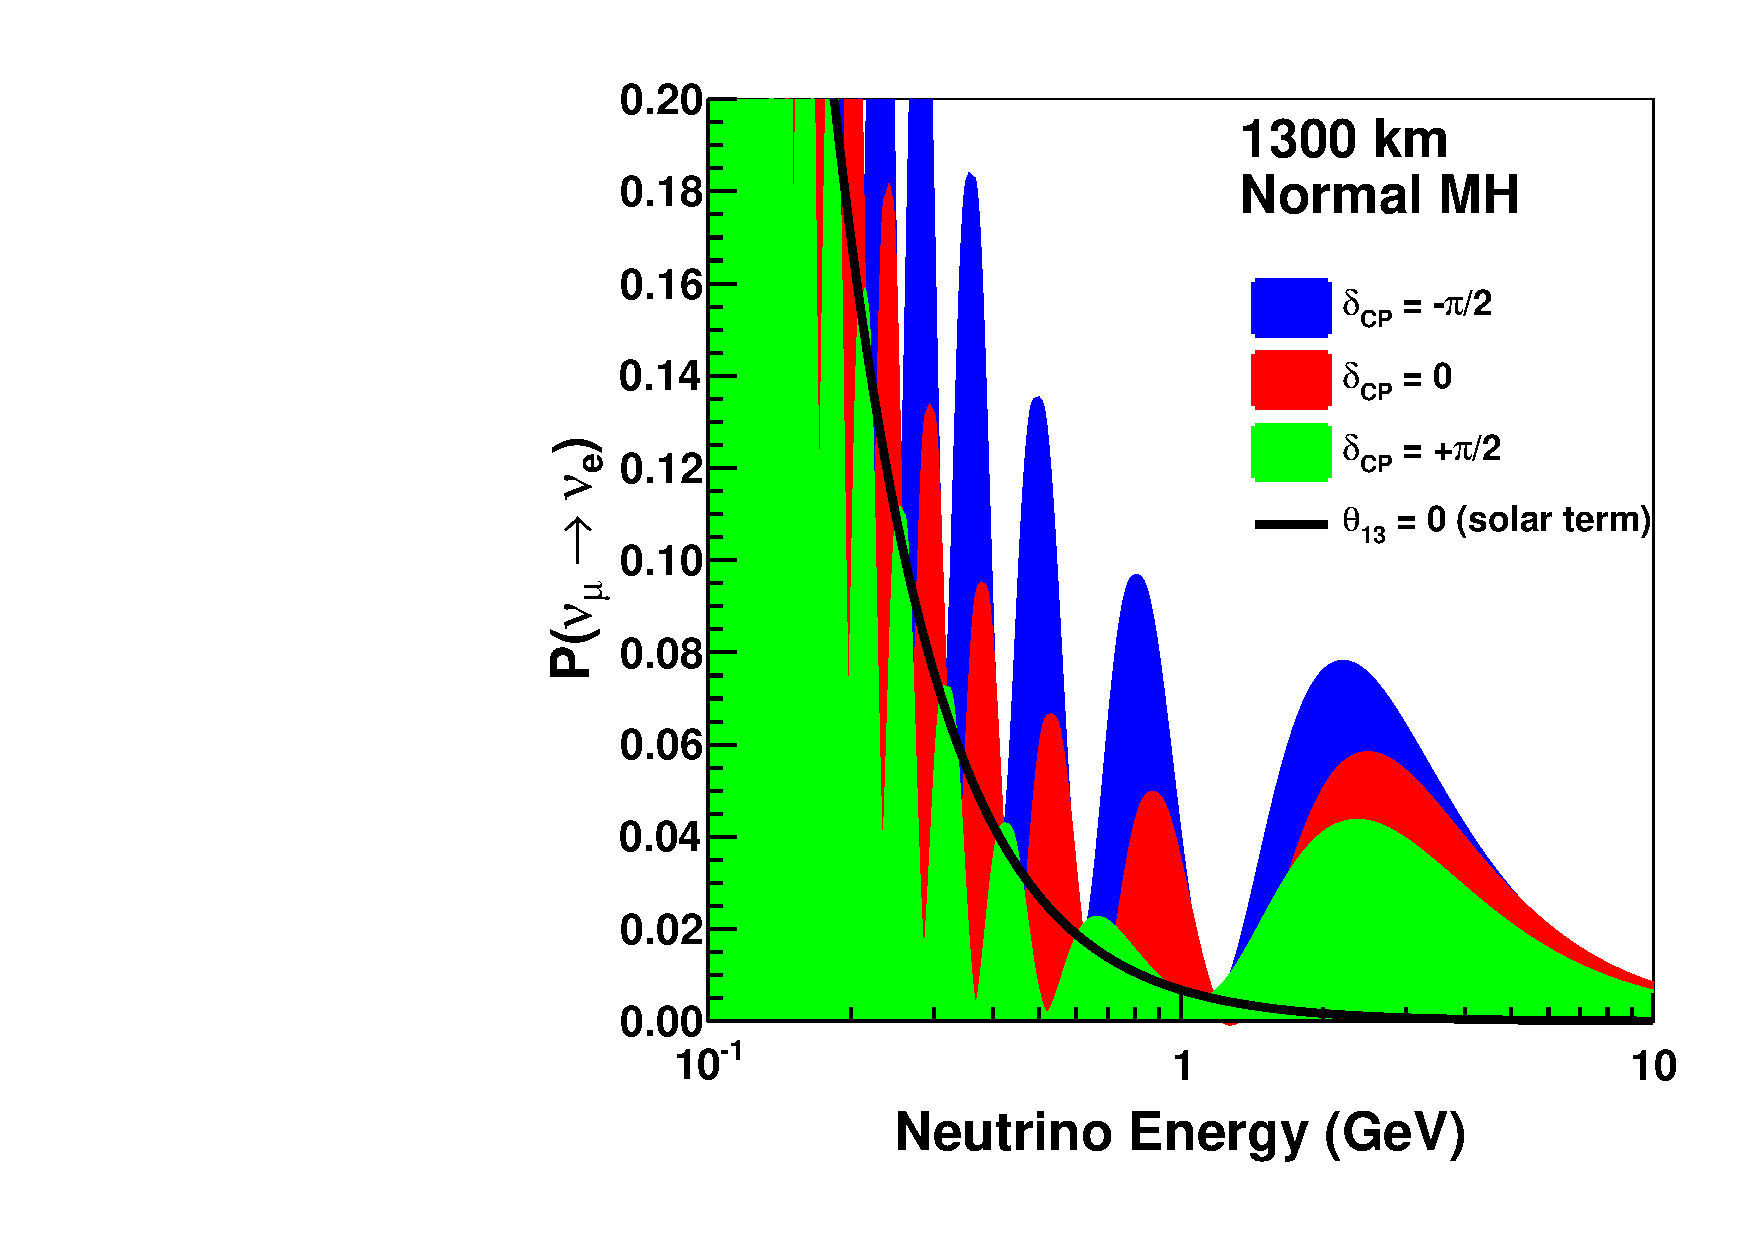
\includegraphics[width=0.55\textwidth]{energy_nu_no}} -- change image file

%\begin{document}

%%%%%%%%%%%%%%%%%%%%  REMOVE ABOVE %%%%%%%%%%%%%%%%%
%\newduneword{rucio}{Rucio}{Data management system originally developed by ATLAS but now open-source and shared across HEP}
%\newduneabbrev{doma}{DOMA}{Data Organization, Management, and Access}{Data Organization, Management, and Access efforts through the HEP Software Foundation}
%\newduneabbrev{hsf}{HSC}{High Energy Physics Software Foundation}{High Energy Physics Software Foundation}
%\newduneabbrev{wlcg}{WLCG}{Worldwide LHC Computing Grid}{Worldwide LHC Computing Grid}
%\newduneabbrev{osg}{OSG}{Open Science Grid}{Open Science Grid}
%\newduneabbrev{sci}{SCI}{Scientific Computing Infrastructure}{Proposed extension of the infrastructure component of \dword{wlcg} to other experiments}
%\newduneabbrev{csc}{CSC}{Computing and Software Consortium}{DUNE Computing and Software Consortium}


\chapter{Computing in DUNE}
\label{ch:exec-comp}
%
%\fixme{Heidi, this outline may be overkill for the exec summary; it may be a good structure for the computing CDR volume, then pared down for inclusion here. My 2 cents! -Anne}
%%%%%%%%%%%%%%%%%%%%%%%%%%%%%%%%%%%%%%%%%%%%%%%%%%%%%%%%%%%
%\section{To remove: just examples}
%\label{sec:exec-comp-1}
%
%Sample figure to copy and edit, Figure~\ref{fig:map}:
%
%\begin{dunefigure}[DUNE collaboration global map]{fig:mhexec}{The international DUNE
%collaboration. Countries with DUNE membership are shown in orange.}
%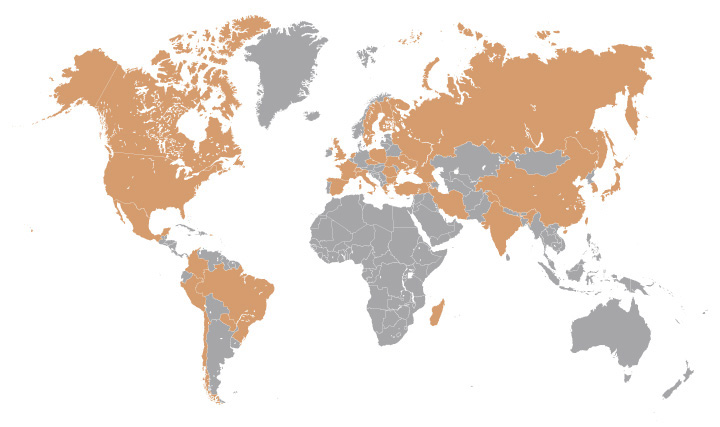
\includegraphics[width=0.9\textwidth]{global-retouched.jpg}  
%\label{fig:map}
%\end{dunefigure}
%
%Sample table to copy and edit, Table~\ref{tab:execosctable}:
%
%\begin{dunetable}[Required exposures to reach oscillation physics
%  milestones]{lcc}{tab:execosctable}{The exposure in mass (kt) $\times$ proton beam power
%    (MW) $\times$ time (years) and calendar years assuming the staging plan described in this chapter needed to reach certain oscillation physics
%    milestones. The numbers are for normal hierarchy using the NuFit 2016 best fit values of the known oscillation parameters.  }
%Physics milestone & Exposure  & Exposure \\ \rowtitlestyle
%  & (\ktMWyr{}) & (years)  \\ \toprowrule 
%  $1^\circ$ $\theta_{23}$ resolution ($\theta_{23} = 42^\circ$) & 29  &  1\\ \colhline
%  CPV at $3\sigma$ ($\delta_{\rm CP} = -\pi/2$)  & 77 &  3\\ \colhline
%  \dword{mh} at  $5\sigma$ (worst point) & 209 & 6 \\ \colhline
%  $10^\circ$ $\delta_{\rm CP}$ resolution ($\delta_{\rm CP} = 0$) & 252 & %5 
%  6.5 \\ \colhline
%  ($\sin^2 2 \theta_{13} = 0.084 \pm 0.003$) &  &  \\  
%\end{dunetable}
%
%%%%%%%%%%%%%%%%%%%%%%%%%%%%%%%%%%%%%%%%
\section{Executive Summary}		
\label{ch:exec-comp-es}







The DUNE long baseline neutrino oscillation collaboration consists of 178 institutions from 32 countries, including 15 European nations and CERN. The experiment is in preparation now with commissioning of the first module expected over the period 2024-2026 and a long data taking run with 4 modules expected from 2026-2036 and beyond.  An active prototyping program is already in place with a short test beam run with a 700T, 15,360 channel prototype of single-phase readout at the neutrino platform \dword{cern} in late 2018 and tests of a similar sized dual-phase detector scheduled for mid-2019.   The DUNE experiment has already  benefited greatly from these initial tests.  The collaboration has recently formed a formal Computing Consortium, with significant participation by European Institutions and interest from groups in Asia to work on common software and computing development and to formalize resource contributions.

The consortium resource model benefits from existing Grid and \dword{wlcg} infrastructure developed for the LHC.  DUNE, through  the ProtoDUNE-SP effort, is already using global resources for simulation and the analysis of ProtoDUNE-SP data.  Multiple European sites are part of this resource pool and are making significant contributions to the ProtoDUNE single and dual phase programs.  We expect this global computing consortium to grow and evolve as we move towards data from the full DUNE detectors in the middle of the next decade.

The DUNE science program is expected to produce raw data volumes similar in scale to the data volumes that current LHC Run-2 experiments have already recorded.  Baseline predictions for the DUNE data, dependent on actual detector performance and noise levels, are 30-60 PB of raw data per year.  These data, with simulations and derived analysis samples, need to be available to all collaborating institutions.  We anticipate that institutions worldwide will play an important role both as contributors and end-users of storage and CPU resources for DUNE.

To enable these resource contributions in cooperation with the LHC and other communities, we plan to utilize common computing layers for infrastructure access and use common tools to ease integration of facilities with both the DUNE and LHC computing ecosystems.  We will use common data storage methodologies to establish large highly available data lakes worldwide  and to collaborate with the broader HEP community in developing other common tools.


HEP has considerable infrastructure in place for international computing collaboration thanks to the LHC program.  Other large experiments - LSST, SKA, DUNE and HyperK will be coming on board over the next decade.   This cooperation is being formalized through the HEP Software Foundation(\dshort{hsf})\lcite{Alves:2017she}, an organization of interested parties working to gather and disseminate common solutions based on the extensive knowledge we have gained over the past two decades. 
DUNE's strategy is to work with and contribute to this global community to maximize the use of common tools for data movement and storage, job control and monitoring, accounting and authentication.   All large-scale experiments will encounter similar issues and worldwide cooperation on common tools is the most cost-effective way to proceed. For example, in collaboration with the Fermilab, CERN and the UK groups, we are investigating the use of {\it \dword{rucio}}  as our primary data manager.

The 2018 test beam run of ProtoDUNE Single-Phase (SP) was a valuable live test of this model.  The ProtoDUNE Single Phase detector at CERN produced raw data at rates of up to ~2GB/s of data.  These data were stored on tape at CERN and Fermilab and replicated at sites in the UK and Czech Republic.  In total 1.8 PB of raw data were produced during the test beam run. 
This prototype run has been extremely beneficial in exercising the existing computing infrastructure and in building a team of interested institutions.


In addition to traditional HEP computational strategies, DUNE's data consists of simple but very large 2D data objects which share many characteristics with astrophysical images.  This presents opportunities to use current advances in machine learning and pattern recognition as a frontier user of High Performance Computing facilities capable of massively parallel processing.  We share this problem, and propose to share solutions, with the other Liquid Argon experiments - ArgoNeut, MicroBooNE, SBND and ICARUS.  We have already benefited greatly from prior work and plan to contribute cooperatively.

In summary, DUNE's computing strategy is to be {\bf global}, working with partners worldwide, and {\bf collaborative}, as almost all of the computational challenges we face are faced by similar experiments. 
 


%%%%%%%%%%%%%%%%%%%%%%%%%%%%%%%%%%%%%%%%
\section{Overview}		
\label{ch:exec-comp-ovr}
The main goal of the computing effort is to facilitate the acquisition, processing and analysis of data and simulations from the DUNE experiment across the many physics drivers for the experiment in a cost effective and secure way. Computing and Software provides the bridge between the real-time online systems of the DUNE/LBNF hardware and the physics groups who develop high-level algorithms and perform data analysis. S+C works with collaborating institutions to identify CPU and storage resources and to support basic software infrastructure such as software frameworks, data catalogs, database infrastructure and code distributions systems. 

The Consortium is currently working with national agencies and major laboratories to negotiate CPU and storage provision for the near term ProtoDUNE runs and development of the full DUNE computing model and is starting the process of evaluating major software infrastructure systems such as workload management, emphasizing collaboration and reuse of existing systems. 

Our initial assessment of needs indicates that data rates and CPU needs for DUNE are significantly less than those for the large LHC experiments but that the extremely large size of individual DUNE events presents unique technical challenges that will require substantial effort to address.  In addition, the collaboration is truly international and will require a distributed computing model to both fully exploit our global computing resources and to make those resources easily available to all collaborators. 


\section{Data types and volumes}
Maximum raw data volumes from the detectors are reasonably easy to estimate, as a product of trigger rate, number of channels, \# of time slices/channel,  size for each ADC readout and compression. However, those data sizes would be well beyond the ability of any system to handle. Thus decisions must be made about what to keep and what not to keep. Those decisions are the purview of the collaboration scientists and the data acquisition design with feedback from computing on what is possible.  The ProtoDUNE experience has provided invaluable information to feed back to the experiment design. 




\subsection{Far detector}

The computing model needs to be able to handle a wide range of data inputs from the far detectors, as documented in more detail in docdb-9240\lcite{bib:docdb9240}.

\begin{itemize}
\item Supernova triggers which would have an uncompressed size of 138 TB for a 30 second readout of all channels in a 4-module single-phase detector at a likely rate of 1/month.  
\item Beam neutrino interactions within a single detector module with an uncompressed size of $\approx$ 6.2 GB at a rate of up to 1 Hz
\item Atmospheric neutrino interactions, nucleon decay and other lower energy processes confined to a subset of a detector module with a low threshold largely driven by radiological backgrounds.
\item Cosmic ray and rock muons at a rate of around 4,500/day/module.
\item Other calibration systems 
\end{itemize}

The estimates in docdb-9240, with conservative estimates for increased needs for low level data taking during commissioning, have led to a negotiated upper limit of 30 PB/year data volume as a standard for both the trigger and data acquisition and computing groups to work towards. 


\begin{dunetable}[Useful quantities for computing estimates]{lrrr}{tab:exec-comp-bigpicture}{Useful quantities for computing estimates}%\rowtitlestyle
Quantity&Value&Units&Explanation\\ 
\hline
{\bf Far Detector Beam:}\\
Single APA readout &41.5& MB& Uncompressed 5.4 ms\\
APAs per module& 150& &\\
Full module readout &6.22&  GB& Uncompressed 5.4 ms\\
Beam rep. rate&\beamreprate& Hz&Untriggered\\
CPU time/event&600-1,200&sec&from MC/ProtoDUNE\\
Memory footprint&2-4&GB&ProtoDUNE experience\\
\hline
{\bf Supernova:}\\
Single channel readout &90.0&MB& Uncompressed 30 s\\
Four module readout&138.2& TB& Uncompressed 30 s\\
Trigger rate&1 & per month&(assumption)\\
%Yearly rates nd
%Reduction with roi.  
%CPU time/ event for reconstruction
%Reduction for analysis
%Users 
\end{dunetable}

\subsection{Near Detector}
In addition, a near detector of reasonable size will have multiple neutrino interactions/beam spill leading to a need to read out at the full beam rate of 0.8-1.2 Hz.
The near detector will have fewer channels and better signal/noise discrimination but much higher readout rates.  While the details of the detector design are still unknown, we assume data volumes of similar size to the far detector (30PB/year) in our planning.

\subsection{Simulation}
The bulk of data collected is likely to be backgrounds, with real high energy events in the far detector numbering in the thousands/year, not millions. Thus the size of simulation samples is likely to be less than that of the raw data.  Lower energy events are either very rare or can be simulated in sub-volumes of the whole detector.  As a result, while simulation will be an important part of the experiment, it is not expected to dominate data volumes as it does in many experiments.  

However, simulation inputs such as flux files, overlay samples and shower libraries pose a special problem as they must be distributed to simulation jobs carefully.  Proper simulation requires that these inputs be delivered in an unbiased fashion. This can be technically difficult in a widely distributed environment and will require thoughtful design. 

\subsection{Analysis}

Analysis formats have not yet been fully defined.  We anticipate that most analysis samples will be orders of magnitude smaller than the raw data.  However, as they are idiosyncratic to particular analyses and in fact particular users,  producing and cataloging them will be sociologically difficult. 
Likely there will be a mix of official samples -  produced by physics groups and distributed through a common catalog and file transfer mechanisms - and user samples on local disk. 


\section{ProtoDUNE-SP as an example}		
\label{ch:exec-comp-proto-SP}
The first ProtoDUNE single phase run at CERN in late 2018 has already led to a small-scale test of a global computing model.  In the following we will describe the ProtoDUNE data design and the lessons learned from our experience. Much of this carries over into planning for full far-detector operations. 

\subsection{Introduction}

The ProtoDUNE Single Phase detector ran at CERN in the np04 beamline from September to November of 2018. Since then, studies with cosmic rays have continued. Prior to that run there were several data challenges at high rate to validate the data transfer mechanisms. 

The first phase of operations was commissioning of the detector readout systems while the argon reached full purity.  Data were taken with cosmic rays and beam during the commissioning period.  Physics data were then taken with beam at full  Argon purity through October and half of November.  Since beam was turned off, cosmic ray data continues to be taken with varying detector conditions, such as modified high voltage and purity and new readout schemes. 



\subsection{Data volumes}
The single-phase ProtoDUNE detector consists of a \dshort{tpc} with  6 Anode Plane Assemblies (\dshort{apa}), photon detectors (\dshort{pd}s) and a Cosmic Ray Tagger (\dshort{crt}). In addition, the np04 beamline is instrumented with hodoscopes and Cerenkov counters to generate beam triggers and random readouts were done at lower rates to collect unbiased cosmic ray information. The data volume from the test beam run was dominated by readout of the \dshort{TPC}.  Each \dshort{apa} has 2,560 channels and reads out 12 bit ADC values at 2 MHz.  During beam running, the detector was triggered on the incoming beam. The nominal readout window during beam running was  3 ms to match the drift time at the full voltage of 180 kV that was maintained for most of the run.  The total size of the \dshort{tpc} data without compression was thus 138 MB/event.  Compression was implemented before the October beam physics run, lowering the total size per event from around 180 MB to 75 MB.  

\begin{dunetable}[Data volumes]{lrr}{tab:exec-comp-pd-volumes}{Data volumes  recorded by ProtoDUNE-SP}
Type  & Events & Size\\ %\rowtitlestyle
Raw Beam&8.08 M& 520 TB \\
Raw Cosmics&3.46 M& 271 TB\\
Commissioning&3.86 M& 388 TB\\
Pre-commissioning&13.89 M&641 TB\\
\end{dunetable}

Events were written out in raw files of size 8 GB with each containing of order 100 events. The beam was live for two 4.5 s spills every 32 s beam cycle and data were taken at peak rates of up to 50 Hz (typically 25 Hz) leading to compressed DC rates out of the detector of 400-800MB/sec.  Each beam cycle could therefore produce 1-4  8 GB output files.  In earlier running with uncompressed data, and during an April data challenge, transfer rates of up to 2GB/s were demonstrated over substantial periods. 

Beam stopped in November 12 but cosmic ray studies of the detector continue, some with an increase time window of 7.5 ms to collect more complete tracks/readout.  This raises the compressed event size to around 170 MB.


\subsection{ProtoDUNE-SP data streams}
The ProtoDUNE-SP data consist of multiple sources in addition to the TPC data. One of the major challenges for the offline computing systems is merging of these multiple streams into a coherent whole for analysis.  Table \ref{tab:exec-comp-pd-sources} lists the data sources used and their granularity. 

\begin{dunetable}[Data sources]{lrr}{tab:exec-comp-pd-sources}{Data sources  }
Type & indexed by & destination\\
TPC  & run/event & event data\\
Photon Detector data & run/event & event data\\
Cosmic Ray Tagger & run/event & event data\\
Beamline devices & time-stamp & beam database\\
Detector conditions & time-stamp & slow controls database\\
DAQ configuration & run & files/elisa logbook\\
Run quality & run & human generated spreadsheets\\
Data quality & run/event/time & Data Quality web application\\
File metadata & file & \dword{sam} file database\\
\end{dunetable}

Information about the detector conditions, \dword{daq} configuration and run quality is spread across a number of sources and must be collected and then boiled down into the quantities relevant for offline data analysis.  For example, the Slow Controls system logs detector conditions continually.  Offline analysis needs to know about these data with coarser granularity and then have algorithms capable of using that information. A full conditions database transfer mechanism is being developed but was not available during the run.  As a result, with the exception of beamline information, coarse information is currently added to the \dword{sam} file catalog run by run to allow files with given operating conditions to be easily identified and retrieved. Beam data is stored in the \dword{ifbeam}
database and connected to event data via time stamps.

\section{Reconstruction of ProtoDUNE-SP data}
Thanks to substantial previous effort by the 35T prototype, \dword{microboone} and the liquid argon community, high quality algorithms were already in place to reconstruct the TPC  data.  As a result, a first pass reconstruction of the ProtoDUNE-SP data with beam triggers was completed by early December, less than a month after the end of data taking.

%\subsection{Reconstruction}
%
%The TPC data read from the ProtoDUNE detector includes a waveform for
%each of 15,360 channels. Each waveform is the output of a 12-bit ADC sampling
%at 2~MHz the output voltage of a charge-sensitive amplifier connected to one of
%the TPC Wires. 
%%The most interesting contribution to these signals is the
%charge on the wire induced by the motion of electrons in the TPC.
%There are also deliberate voltage offsets to put the signal in the amplifier
%and ADC ranges and there is noise from the electronics (jitter and pickup)
%and wire motion. Finally, each ADC channel has response nonlinearity and
%distortions.
\ignore{
The electrons produced in the \dword{tpc} volume drift % away from a cathode plane
toward three planes of anode wires with voltage bias such that the electrons
pass through the first two planes (called induction planes) and are collected
on the last (collection plane).
The signal induced on the collection plane wires is unipolar 
and the pedestal-subtracted area of the signal is roughly proportional to the
charge collected on that wire.
The signals on the induction wires are bipolar: first a positive signal is produced as
electrons approach the plane and then negative as they move away.
}
%The time (i.e. waveform sample) at which the signal appears provides a measure of the drift
%time which is used to deduce the drift distance.
\subsection{Data preparation}

Before pattern recognition, data from the ProtoDUNE detector is
unpacked and copied to a standard format.
The same format is produced in detector simulation.
This reformatted raw data includes the waveform for each channel, an
integer in the range [0, 4095] for each of 6000-15,000 time slices. 

The first step in reconstruction is data preparation with the goal of
converting each ADC waveform into a calibrated charge waveform with
signals proportional to charge. At the end of data preparation, regions of interest (ROIs), i.e. blocks of contiguous samples where
useful signals appear, are identified and the data outside these regions are discarded.

%Perhaps most important, the bipolar signals in induction wires are made unipolar.
%Also the electronics shaping is replaced with the Gaussian shaping expected in the
%next stage of processing.
%Relative channel-to-channel and absolute calibration is applied to account for the
%responses of the amplifiers and ADCs.
%And attempts are made to remove noise and mitigate ADC distortions.

The sequence is described more fully in docdb-12349\lcite{ref:docdb12349} and in the Methods section of the Physics Volume but is summarized here:

\begin{enumerate}
\item Each waveform is unpacked into integers.
\item Pedestals are determined per event/per channel from the most common ADC value. 
\item Pedestals and calibrations are applied. %\label{local:ped}
\item Bad channels, sticky bits and other know hardware problems are corrected or removed.
\item Signal undershoot that creates a long negative tail is removed. 
\item The waveforms  are deconvoluted.  In the first processing this was done with simple 1-D convolution for a single wire but in future the 2-D convolution described by the MicroBooNE collaboration in \lcite{Adams:2018dra} will be used to eliminate cross-talk with adjacent wires.  The deconvolution Fourier transforms the waveform, applies a response function, applies a low pass filter to remove high frequency noise and then transforms back.



\item Finally regions of interest are defined where the signal exceeds a given threshold and time slices well outside the ROI are dropped, leading to significant reduction in the size of the remaining data. These data are then fed into the reconstruction algorithms for further pattern recognition. %\label{local:roi}
\end{enumerate}




%\subsection{Signal processing}
Figures~\ref{fig:ch-exec-comp-chtraw}-\ref{fig:ch-exec-comp-chtroi} illustrate the transformation of TPC data  during data
preparation.

\begin{figure}[t]
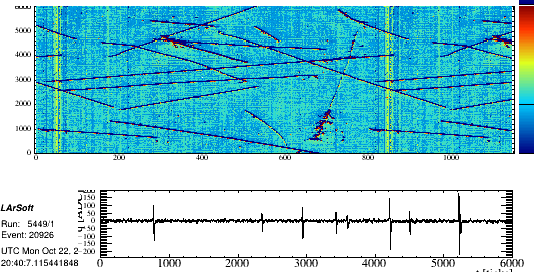
\includegraphics[width=\textwidth,angle=0]{comp-evd_twq-proj_5449_20926_raw.png}
\caption{
Example of pedestal-subtracted data for one of the ProtoDUNE  wire planes.  The top pane shows the ADC values in a V (induction) plane with the x-axis being channel number and the y-axis, time slice. The bottom pane shows the bipolar pulses induced on one channel. 
}
\label{fig:ch-exec-comp-chtraw}
\end{figure}




%\begin{figure}[t]
%  \includegraphics[width=\textwidth]{ccomp-evd.twq-proj.5449.20926.recon..png}
%\caption{
%Same as Fig.~\ref{fig:ch-exec-comp-chtraw} except after hit correction, tail removal and deconvolution.
%}
%\label{fig:ch-exec-comp-chtdco}
%\end{figure}

\begin{figure}[t]
  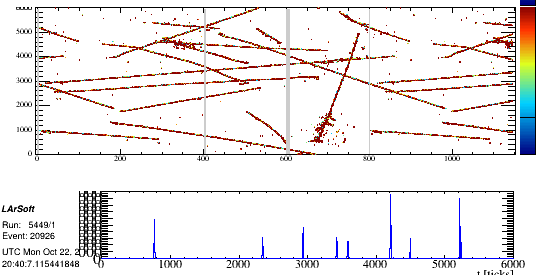
\includegraphics[width=\textwidth]{comp-evd_twq-proj_5449_20926_decon.png}
\caption{
Same as Fig.~\ref{fig:ch-exec-comp-chtraw} except after calibration, cleanup, deconvolution and ROI finding. 
}
\label{fig:ch-exec-comp-chtroi}
\end{figure}

%%%%%%%%%%%%%%%%%%%%%%%%%%%%
%\todo{Statement about timing and memory for this phase}

\subsection{Computational characteristics of data preparation and deconvolution }
Decoding for ProtoDUNE-SP is currently done with all 6 APAs in memory. As each 3 ms APA readout consists of over 15M 12 bit values, decompression and conversion to floating point results in substantial memory expansion.  Decoding and deconvolution of 6 APAs with 3 ms readout fits within a normal 2 GB memory/core footprint but the 7.5 ms readout window used in some cosmic ray studies requires a correspondingly larger memory footprint. As electrical signals are correlated between channels within an APA wire plane, but not between planes, better memory performance can be achieved by processing each wire plane (3/APA) independently. These changes are being implemented.


However,  while subdividing the detector into wire planes solves the memory problems for short readouts it is  not a viable solution for the long readouts expected for supernova events. We are still exploring the best strategy for dealing with these much larger ($\times 10,000$)time windows. The DAQ group is already testing 1 second ($300 \times$ longer time window) readouts of small numbers of channels.  These are being used as tests of optimal models for data segmentation.  Section \ref{ch:exec-comp-mod} describes the start of a bottoms-up collaboration with the \dshort{daq} consortium on an optimal data model for the full DUNE detectors. 

\subsection{Further reconstruction}
The downstream pattern recognition steps starting with \dword{roi} are described further in the Tools and Methods chapter of the Physics Volume.  
Full reconstruction of ProtoDUNE-SP interactions, with beam particles and of order 20-40 cosmic rays per readout window took 600-1200 sec/event.
Table  \ref{tab:comp-raw-data-size} shows the input datasize for a typical beam event, dominated by around 71 MB of TPC waveform information. Table  \ref{tab:comp-reco-data-size} shows the size of different reconstructed objects, still dominated by around 10 MB of reduced TPC hit information,  while \ref{tab:comp-reco-data-time} shows the reconstruction time breakdown.  This event had a 3 ms readout window.  The input size and reconstruction time scale reasonably linearly with the readout window.  

\subsection{Reconstruction characteristics}

The data preparation phase can be segmented by detector component, for example into wire planes within a APA  The operations performed in signal processing require few decisions to be made but do include operations such as fast-Fourier transforms and deconvolution.  These operations are well suited to GPU's. 

Once ROI's have been identified, several 3-D reconstruction packages are used. For the first reconstruction pass in November, the  \dword{pandora}\cite{Acciarri:2017hat}, \dword{wirecell}\cite{wirecell} and \dword{pma}\cite{ref:PMA}  frameworks were used with results described in the Physics volume.   Table \ref{tab:comp-reco-data-time} indicates that they are comparable in terms of CPU time used.   Deep Learning techniques based on image pattern recognition algorithms are also being developed. Many of these algorithms can be adapted to run on HPC's, but probably different architectures that would be optimal for the data preparation phase. 

All of these algorithms are currently being run on conventional unix CPU's using \dword{osg}/\dword{wlcg} grid computing  infrastructure. 



\begin{dunetable}[Compressed size for Raw data - 7 GeV beam events with a 3 ms time window]{rrl}{tab:comp-raw-data-size}{Compressed size for Raw data - 7 GeV beam events with a 3 ms time window}
Size in Kbytes	&	Fraction	&	Data Product Name	\\
\hline
44,155.47	&	0.576	&	artdaq::Fragments\_daq\_ContainerTPC\_DAQ.	\\
27,952.64	&	0.364	&	artdaq::Fragments\_daq\_ContainerFELIX\_DAQ.	\\
4,586.82	&	0.06	&	artdaq::Fragments\_daq\_ContainerPHOTON\_DAQ.	\\
5.72	&	0	&	artdaq::Fragments\_daq\_ContainerCTB\_DAQ.	\\
0.17	&	0	&	artdaq::Fragments\_daq\_TIMING\_DAQ.	\\
0.09	&	0	&	art::TriggerResults\_TriggerResult\_\_DAQ.	\\
\hline
76,703.25 & 1.0 & Total\\
\end{dunetable}

\begin{dunetable}
[Compressed size for Reconstructed data - 7 GeV beam event]
{rrl}
{tab:comp-reco-data-size}
{Compressed size for Reconstructed data - 7 GeV beam events}
Size in kBytes&	Fraction&		Data Product Name	\\
4,218,536	&	0.185	&	recob::Wires\_digitwire\_\_DecoderandReco.	\\
2,236,432	&	0.098	&	recob::Hits\_hitpdune\_\_DecoderandReco.	\\
2,102,520	&	0.092	&	recob::Hits\_gaushit\_\_DecoderandReco.	\\
2,052,796	&	0.090	&	recob::Hits\_linecluster\_\_DecoderandReco.	\\
2,020,575	&	0.089	&	artdaq::Fragments\_daq\_ContainerPHOTON\_DAQ.	\\
1,532,502	&	0.067	&	raw::OpDetWaveforms\_ssprawdecoder\_internal\_DecoderandReco.	\\
1,018,088	&	0.045	&	anab::Calorimetrys\_pandoracalo\_\_DecoderandReco.	\\
873,797&	0.038	&	recob::Tracks\_pandoraTrack\_\_DecoderandReco.	\\
806,513&	0.035	&	anab::Calorimetrys\_pmtrackcalo\_\_DecoderandReco.	\\
555,775&	0.024	&	recob::SpacePoints\_pandora\_\_DecoderandReco.	\\
479,599&	0.021	&	recob::Tracks\_pmtrack\_\_DecoderandReco.	\\
414,824&	0.018	&	raw::OpDetWaveforms\_ssprawdecoder\_external\_DecoderandReco.	\\
391,791&	0.017	&	recob::Hitrecob::Trackrecob::TrackHitMetaart::Assns\_pmtrack\_\_DecoderandReco.	\\
379,553&	0.017	&	recob::SpacePoints\_pmtrack\_\_DecoderandReco.	\\
310,021&	0.014	&	recob::SpacePoints\_reco3d\_pre\_DecoderandReco.	\\
260,143&	0.011	&	recob::Hitrecob::SpacePointvoidart::Assns\_hitpdune\_\_DecoderandReco.	\\
250,175&	0.011	&	recob::Hitrecob::SpacePointvoidart::Assns\_reco3d\_\_DecoderandReco.	\\
229,711&	0.01	&	recob::SpacePoints\_reco3d\_noreg\_DecoderandReco.	\\
218,874&	0.01	&	recob::SpacePoints\_reco3d\_\_DecoderandReco.	\\
200,618&	0.009	&	recob::Hitrecob::SpacePointvoidart::Assns\_pandora\_\_DecoderandReco.	\\
2,407,376&0.106	&Smaller Objects	\\
\hline
22,759,597&	1.000		&Total	\\
\end{dunetable}

<<<<<<< HEAD
\begin{dunetable}[Algorithm timing for 7 GeV beam event]{lrr}{tab:comp-reco-data-time}{Algorithm timing for 7 GeV beam events.  Smaller processes not shown for clarity. A 10 event job used 2.7 GB of memory to do this reconstruction.}
Processing step&Average CPU time, sec\\									
source:RootInput(read)	&	0.2	\\
%decode:timingrawdecoder:TimingRawDecoder	&	0.0	\\
%decode:ssprawdecoder:SSPRawDecoder	&	0.3	\\
decode:tpcrawdecoder:PDSPTPCRawDecoder	&	15.9	\\
%decode:crtrawdecoder:CRTRawDecoder	&	0.0	\\
%decode:ctbrawdecoder:PDSPCTBRawDecoder	&	0.0	\\
decode:beamevent:BeamEvent	&	0.7	\\
decode:caldata:DataPrepModule	&	89.1	\\
decode:wclsdatasp:WireCellToolkit	&	113.3	\\
%decode:digitwire:EventButcher	&	0.8	\\
decode:gaushit:GausHitFinder	&	20.7	\\
decode:reco3d:SpacePointSolver	&	18.0	\\
decode:hitpdune:DisambigFromSpacePoints	&	23.0	\\
decode:linecluster:LineCluster	&	3.9	\\
decode:pandora:StandardPandora	&	93.2	\\
decode:pandoraTrack:LArPandoraTrackCreation	&	12.3	\\
decode:pandoraShower:LArPandoraShowerCreation	&	5.2	\\
decode:pandoracalo:Calorimetry	&	5.8	\\
%decode:pandorapid:Chi2ParticleID	&	0.0	\\
decode:pmtrack:PMAlgTrackMaker	&	142.0	\\
decode:pmtrackcalo:Calorimetry	&	6.1	\\
%decode:pmtrackpid:Chi2ParticleID	&	0.0	\\
%decode:ophitInternal:OpHitFinder	&	0.0	\\
%decode:ophitExternal:OpHitFinder	&	0.0	\\
%decode:opflashInternal:OpFlashFinder	&	0.0	\\
%decode:opflashExternal:OpFlashFinder	&	0.0	\\
%[art]:TriggerResults:TriggerResultInserter	&	0.0	\\
%end_path:out1:RootOutput	&	0.0	\\
cout1:RootOutput(write)	&	3.3\\	
Total&	503.7\\
\end{dunetable}
=======
\begin{dunetable}[Reconstruction times for 7 GeV beam event]{lrr}{tab:comp-raw-data-size}{Reconstruction times for 7 GeV beam events}
Processing step &	Avg CPUtime(sec) 	\\			
\hline			
Fullevent	&	503.7	\\
\hline			
source:RootInput(read)	&	0.2	\\
%decode:timingrawdecoder:TimingRawDecoder	&	0.0	\\
decode:ssprawdecoder:SSPRawDecoder	&	0.3	\\
decode:tpcrawdecoder:PDSPTPCRawDecoder	&	15.9	\\
%decode:crtrawdecoder:CRTRawDecoder	&	0.0	\\
%decode:ctbrawdecoder:PDSPCTBRawDecoder	&	0.0	\\
decode:beamevent:BeamEvent	&	0.7	\\
decode:caldata:DataPrepModule	&	89.1	\\
decode:wclsdatasp:WireCellToolkit	&	113.3	\\
decode:digitwire:EventButcher	&	0.8	\\
decode:gaushit:GausHitFinder	&	20.7	\\
decode:reco3d:SpacePointSolver	&	18.0	\\
decode:hitpdune:DisambigFromSpacePoints	&	23.0	\\
decode:linecluster:LineCluster	&	3.9	\\
decode:pandora:StandardPandora	&	93.2	\\
decode:pandoraTrack:LArPandoraTrackCreation	&	12.3	\\
decode:pandoraShower:LArPandoraShowerCreation	&	5.2	\\
decode:pandoracalo:Calorimetry	&	5.8	\\
decode:pandorapid:Chi2ParticleID	&	0.0	\\
decode:pmtrack:PMAlgTrackMaker	&	142.0	\\
decode:pmtrackcalo:Calorimetry	&	6.1	\\
%decode:pmtrackpid:Chi2ParticleID	&	0.0	\\
%decode:ophitInternal:OpHitFinder	&	0.0	\\
%decode:ophitExternal:OpHitFinder	&	0.0	\\
%decode:opflashInternal:OpFlashFinder	&	0.0	\\
%decode:opflashExternal:OpFlashFinder	&	0.0	\\
%[art]:TriggerResults:TriggerResultInserter	&	0.0	\\
%end_path:out1:RootOutput	&	0.0	\\
:out1:RootOutput(write)	&	3.3	\\\end{dunetable}
>>>>>>> 0409f6327748e16759137f14bdf97ff9e368f272





 




\section{Processing Infrastructure for Reconstruction and Simulation}
\label{ch-comp-processing}
ProtoDUNE makes use of computing resources internationally through the Open Science Grid and the parallel infrastructure set up for WLCG in Europe.  In 2018, significant effort was put into integrating European sites into the DUNE reconstruction and simulation processing with very positive results.  
Figure \ref{fig:ch-exec-comp-cpupie} shows the distribution of production jobs worldwide in November and December 2018 during the main reconstruction pass.  FNAL and CERN as the host laboratories made the largest contributions but significant resources were also made available from the UK through integration with GridPP and in the Czech republic through FZU and at IN2P3 in France. 

\begin{figure}[htp]
\centering
%\subfloat[]{
%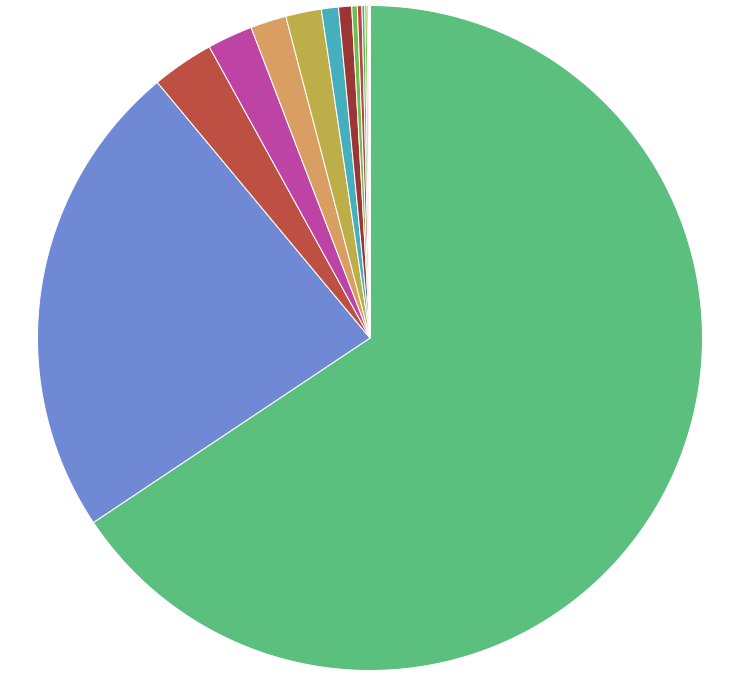
\includegraphics[height=2.5in]{comp-dunepro_pdsp_keepup.png}%
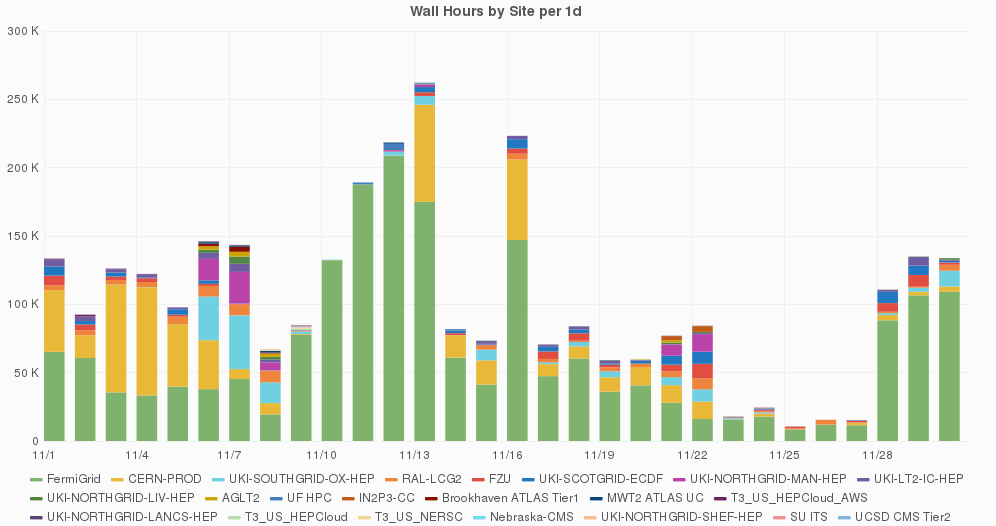
\includegraphics[height=4in]{graphics/comp-vo-summary.png}
%}
%\vspace{1cm}
%\subfloat[]{
%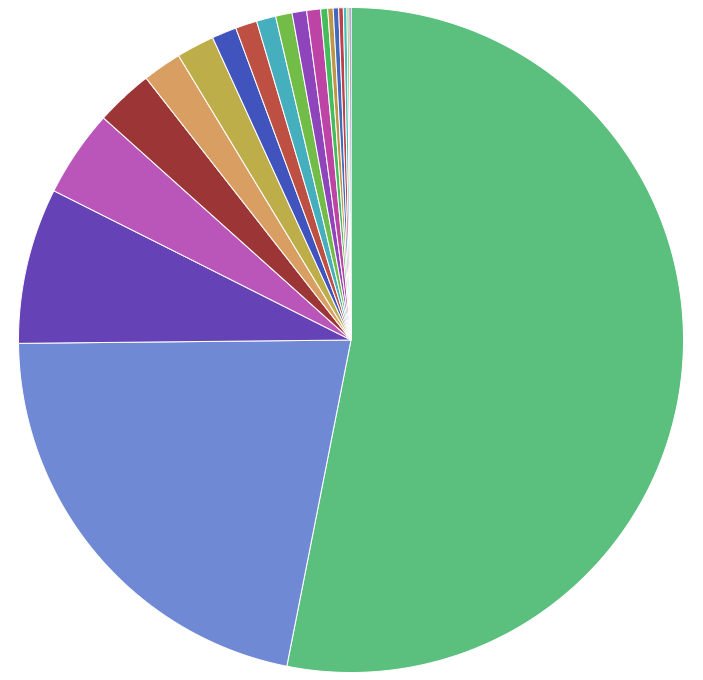
\includegraphics[height=2.3in]{comp-dunepro_mcc11.png}%
%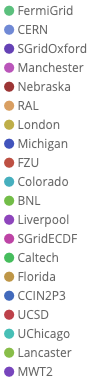
\includegraphics[height=2.3in]{comp-dunepro_mcc11_legend.png}
%}
\caption{CPU wall-time for November 2018 during ProtoDUNE-SP reconstruction showing multiple site contributions.  The major contributions were from FNAL, CERN, many UK institutions and FZU.}
\label{fig:ch-exec-comp-cpupie}
\end{figure}

\begin{dunetable}
[Data storage  and CPU needs for reconstruction of ProtoDUNE test beam data]
{llrrrr}{tab:exec-comp-needs}{Data storage and CPU needs for reconstruction of ProtoDUNE-SP test beam data taken in 2018 and projections for 2019-2021.  We assume two copies of raw data are stored and that each event is reconstructed twice.  Analysis and simulation are estimated to be of order the same CPU use as reconstruction based on the 2018 experience.}%\rowtitlestyle
Detector& value &
2018&
2019&
2020&
2021\\
&&As built\\
\hline
SP&
Events, M&
15.1&
13.0&
6.5&
40.5\\
&
Raw data, TB&
1047&
2239&
1120&
2799\\
&
Reco data, TB&
2094&
4479&
2239&
5599\\
&
CPU, MH&
5.0&
4.3&
2.2&
13.5\\
\hline
DP&
Events, M&
0.0&
101.1&
56.2&
119.9\\
&
Raw data, TB&
0&
809&
449&
1799\\
&
Reco data, TB&
0&
1617&
899&
3598\\
&
CPU, MH&
0.0&
33.7&
18.7&
40.0\\
\hline
total&
Events, M&
15.1&
114.0&
62.6&
160.4\\
&2x
Raw data, TB&
2094&
6096&
3138&
9197\\
&
Reco data, TB&
2094&
6096&
3138&
9197\\
total&Storage, TB
4188&
12193&
6276&
18394\\
&
Reco CPU, MH&
5.0&
38.0&
20.9&
53.5\\
&
Analysis CPU, MH&
5.0&
40.0&
40.0&
40.0\\
Total&CPU, MH&
10.0\\
78.0\\
60.9\\
93.5\\
\end{dunetable}

\subsection{Lessons learned}

\begin{itemize}
    \item Data and simulation challenges led to a reasonably mature and robust model for acquiring, storing and cataloging the main data stream. 
    \item The experiment was able to integrate multiple existing grid sites and make use of substantial opportunistic resources.  This allowed initial processing of data within one month of the end of the run.
    \item Substantial but successful effort went into signal processing. 
    \item Reconstruction algorithms are not perfect but sufficient for studies of detector performance and calibration. 
    \item Beam information was successfully integrated into the processing through the \dword{ifbeam} database.
    \item Auxiliary information from, for example, slow controls was not integrated into processing due to lack of personpower.  This led to dependence on hand input of running conditions by shift personnel and offline incorporation of that information into the data catalog. 
\end{itemize}

Overall, the ProtoDUNE-SP data taking and processing was a success but overly dependent on doing things "by hand" as automated processes were not always in place. 

\subsection{Near future}

Table \ref{tab:exec-comp-needs} summarizes the known resource usage for 2018 and projections for 2019-2021.  The collaboration has requested a substantial test beam run for both single and dual phase detectors in 2021.  The \dshort{csc} views this run as a first production test for the full DUNE computing infrastructure. 





%%%%%%%%%%%%%%%%%%%%%%%%%%%%%%%%%%%%%%%%
\section{Data Model for the Far and Near Detectors}		
\label{ch:exec-comp-mod}

%%%%%%%%%%%%%%%%%%%%
\subsection{Introduction}	
\label{ch:exec-comp-mod-int}
In parallel with the ProtoDUNE-SP data, a joint Data Model task force was formed by the DAQ and Computing Consortia to lay a framework for the full near and far DUNE detectors. 
The Data Model task force grappled with the problems of efficiently triggering, reading out and storing data from an enormous detector on multiple time scales.

They defined major concepts.

\begin{description}

\item{Configuration:} set of parameters that define the persisted, expected detector state. Globally, this corresponds to a desirable state for the detector, capable of providing data of physics or calibration quality. Each component of the detector may have its own configuration.
 
\item{Run:} Period of time over which data has been collected across some set of desired components in a consistent configuration.
 
\item{Subrun:} Period of time within a run over which data has been collected across some set of desired components in a consistent configuration. The set of desired components in a subrun must be a subset of the desired components for a run, and is the set of components over which data is expected.
 
(Time-based rollovers of runs and subruns may be automatic. Differences of subrun and run due to configuration or changes in the desired components will be tracked by the DAQ, and may be either manual or automatic.)
 
\item{Trigger:} data from the desired components in that subrun over a window of time (a ?readout window?). This would typically be centered around a trigger time, and is what is recorded by the DAQ. The readout window may be subdivided into ?frames? as determined by the DAQ.
 
\item{Event:} subset of a trigger isolated in time and space containing an independent interaction in the detector. Events may overlap in space or time, within the same trigger. This is generally determined by the offline, based on reconstruction of data in a frame.

\end{description}

These definitions are intended to allow triggering, recording and reconstruction of interactions in subsets of the detector. While the whole detector (or time window) can produce enormous amounts of data, any individual interaction is expected to span a reasonably short time and spatial volume. A data model that can isolate individual interactions  allows efficient storage and reconstruction of interactions. 


The main data stream will be augmented by beam, slow controls, \dword{daq} configuration and calibration information. 

This work continues and informs  the  joint  calibration, \dshort{csc} and \dshort{daq} designs.


\section{Consortium Organization}

%The DUNE computing and software consortium was formed in October 2018.  
%%%%%%%%%%%%%%%%%%%%
%\subsection{Requirements}	
%\label{ch:exec-comp-mod-req}


%%%%%%%%%%%
%\subsubsection{How Physics Drives}
%\label{ch:exec-comp-mod-req-phys-drv}


%%%%%%%%%%%
%\subsubsection{Oscillation Analyses}
%\label{ch:exec-comp-mod-req-osc}


%%%%%%%%%%%
%\subsubsection{Cross Sections}
%\label{ch:exec-comp-mod-req-xsec}


%%%%%%%%%%%
%\subsubsection{Other Drivers}
%\label{ch:exec-comp-mod-req-oth-drv}


%%%%%%%%%%%%%%%%%%%%
%\subsection{Interfaces with Other Projects}	
%\label{ch:exec-comp-mod-intfc}


%%%%%%%%%%%
%\subsubsection{DAQ}
%\label{ch:exec-comp-mod-intfc-daq}


%%%%%%%%%%%
%\subsubsection{Calibration}
%\label{ch:exec-comp-mod-intfc-calib}

%Why is this cutting off here on the page?

%%%%%%%%%%%
%\subsubsection{Physics}
%\label{ch:exec-comp-mod-intfc-phys}

%Why is this cutting off here on the page?

%%%%%%%%%%%%%%%%%%%%
%\subsection{Use cases}	
%\label{ch:exec-comp-mod-use}


%%%%%%%%%%%
%\subsubsection{Discussion of detector options (SP,DP,ND? )}
%\label{ch:exec-comp-mod-use-opt}


%%%%%%%%%%%
%\subsubsection{Data acquisition}
%\label{ch:exec-comp-mod-use-daq}


%%%%%%%%%%%
%\subsubsection{Data Quality}
%\label{ch:exec-comp-mod-use-dq}


%%%%%%%%%%%
%\subsubsection{Reconstruction}
%\label{ch:exec-comp-mod-use-reco}


%%%%%%%%%%%
%\subsubsection{Calibration}
%\label{ch:exec-comp-mod-use-calib}


%%%%%%%%%%%
%\section{Simulation}
%\label{ch:exec-comp-mod-use-sim}


%%%%%%%%%%%
%\section{Analysis}
%\label{ch:exec-comp-mod-use-anls}


%%%%%%%%%%%%%%%%%%%%
%\subsection{Existing Infrastructure}	
%\label{ch:exec-comp-mod-infr}


%%%%%%%%%%%
%\subsubsection{sam/enstore/eos/castor}
%\label{ch:exec-comp-mod-infr-stor}


%%%%%%%%%%%
%\subsubsection{Grid}
%\label{ch:exec-comp-mod-infr-gr}


%%%%%%%%%%%
%\subsubsection{Databases}
%\label{ch:exec-comp-mod-infr-db}


%%%%%%%%%%%%%%%%%%%%
%\subsection{ProtoDUNE Experience}	
%\label{ch:exec-comp-mod-pdune}


%%%%%%%%%%%%%%%%%%%%
%\subsection{Evolving Infrastructure}	
%%\label{ch:exec-comp-mod-evlv}
%Why is this cutting off here on the page?

%%%%%%%%%%%
%\subsubsection{rucio}
%\label{ch:exec-comp-mod-evlv-ruc}
%Why is this cutting off here on the page?

%%%%%%%%%%%
%\subsubsection{Load Management}
%\label{ch:exec-comp-mod-evlv-load}


%%%%%%%%%%%
%\subsubsection{?.}
%\label{ch:exec-comp-mod-evlv-}


%%%%%%%%%%%%%%%%%%%%
%\subsection{Novel Architectures}	
%\label{ch:exec-comp-mod-nov}

%%%%%%%%%%%
%\subsubsection{HPC}
%\label{ch:exec-comp-mod-nov-hpc}

%%%%%%%%%%%%%%%%%%%%
%\subsection{Authentication}	
%\label{ch:exec-comp-mod-auth}


%%%%%%%%%%%%%%%%%%%%%%%%%%%%%%%%%%%%%%%%
%\section{Software}		
%\label{ch:exec-comp-sw}


%%%%%%%%%%%%%%%%%%%%
%\subsection{Introduction}	
%\label{ch:exec-comp-sw-int}


%%%%%%%%%%%%%%%%%%%%
%\subsection{Existing Packages}	
%\label{ch:exec-comp-sw-int-pkg}


%%%%%%%%%%%
%\subsubsection{GEANT4}
%\label{ch:exec-comp-sw-int-gnt}


%%%%%%%%%%%
%\subsubsection{ROOT}
%\label{ch:exec-comp-sw-int-root}
%hy is this cutting off here on the page?

%%%%%%%%%%%
%\subsubsection{art}
%\label{ch:exec-comp-sw-int-art}


%%%%%%%%%%%%%%%%%%%%
%\subsection{Evolving Packages}	
%\label{ch:exec-comp-sw-evpkg}


%%%%%%%%%%%
%\subsubsection{LArSoft}
%\label{ch:exec-comp-sw-evpkg-larsoft}


%%%%%%%%%%%
%\subsubsection{Wirecell}
%\label{ch:exec-comp-sw-evpkg-wcell}


%%%%%%%%%%%
%\subsubsection{GENIE}
%\label{ch:exec-comp-sw-evpkg-genie}


%%%%%%%%%%%%%%%%%%%%
%\subsection{DUNE-specific Software}	
%\label{ch:exec-comp-sw-evpkg-spec}


%%%%%%%%%%%%%%%%%%%%
%\subsection{Novel Architectures}	
%\label{ch:exec-comp-sw-novarch}

%%%%%%%%%%%
%\subsubsection{Machine Learning}
%\label{ch:exec-comp-sw-novarch-mach}
%Why is this cutting off here on the page?
%%%%%%%%%%%
%\subsubsection{Vectorization}
%\label{ch:exec-comp-sw-novarch-vec}

%%%%%%%%%%%%%%%%%%%%
%\subsection{Development Environment	}
%\label{ch:exec-comp-sw-devenv}

%%%%%%%%%%%
%\subsubsection{Environment Specifications}
%\label{ch:exec-comp-sw-devenv-spec}


%%%%%%%%%%%
%\subsubsection{Code and Configuration Management}
%\label{ch:exec-comp-sw-devenv-mgmt}


%%%%%%%%%%%
%\subsubsection{Validation}
%\label{ch:exec-comp-sw-devenv-val}


%%%%%%%%%%%%%%%%%%%%
%\subsection{Training and Communication}	
%\label{ch:exec-comp-sw-train}
%Why is this cutting off here on the page?

%%%%%%%%%%%%%%%%%%%%
%\subsection{Lessons from ProtoDUNE}	
%\label{ch:exec-comp-sw-lessons}


%%%%%%%%%%%%%%%%%%%%%%%%%%%%%%%%%%%%%%%%
\section{Resources and Governance}		
\label{ch:exec-comp-gov}

The Computing and Software effort is now a DUNE Consortium.  Docdb 12751 \lcite{bib:docdb12751} describes the governance structure for the Consortium.  The Consortium coordinates effort across the collaboration but funding comes from collaborating institutions, laboratories and national funding agencies. 

The consortium has an overall Consortium Leader. The Consortium Leader is responsible for the sub-system deliverables and represents the consortium to the overall DUNE collaboration.

In addition there  are Technical Leads to act as the overall project managers for the consortium. The Technical Leads report to the overall Consortium Leader.
Computing has both a Host Laboratory Technical Project Lead, responsible for coordination with the DUNE Project and host lab and an International Technical Lead responsible for coordination with institutions outside the US.?
As with other DUNE consortia, the consortium is responsible for assigning a provisional division of institutional
responsibilities for computing resources, deliverables and operations, amongst the participating institutions. This division of responsibilities must account for the resources that are likely to be available. The internally agreed division of responsibilities needs to be presented to the Technical Board, which will then make a recommendation to the collaboration management for approval.



\subsection{Scope of the Consortium}
The Computing and Software Consortium (\dword{csc}) is mainly concerned with the infrastructure and resources for offline computing.  Algorithm development resides within the Physics groups while online systems at experimental sites are governed by the Data Acquisition and Cryogenics Instrumentation and Slow Controls Consortia. These groups coordinate closely to assure that the full chain of data acquisition, processing and analysis works. Formal interfaces with these groups are described in Docdb 7123 (DAQ)\lcite{bib:docdb7123} and Docdb 7126 (CISC)\lcite{bib:docdb7126}.

The consortium operates at two levels; at the hardware level, where generic resources can be provided as in kind contributions to the collaboration and at the human level, where individuals and groups contribute to the development of common software infrastructure. 

\subsection{Hardware}
As noted above, the collaboration has already made use of substantial global resources through the \dword{wlcg} and \dword{osg} grid mechanisms. As the Consortium evolves, institutions and collaborating nations will be asked to make formal pledges of resources (both CPU and storage) and those resources will be accounted for and considered in-kind contributions to the collaboration.
As illustrated above, several international partners are already making substantial contributions. We are currently integrating additional large national facilities. Most resources are currently opportunistic but Fermilab and CERN have committed several thousand cores and several PB of disk and the UK reserves 10\% of GridPP resources for non-LHC experiments, an allocation that DUNE has already benefited from.

\begin{dunetable}
[DUNE S+C Consortium Members as of February 20 19]{lll}{tab:exec-comp-consortium}{DUNE S+C Consortium Members as of February 2019, -- indicates sites not yet integrated into production computing. }%\rowtitlestyle
Institution& Country & Integrated\\
KISTI	&	Korea	&	--	\\
Nikhef	&	NL	&	Yes	\\
Edinburgh	&	UK	&	Yes	\\
GridPP	&	UK	&	Yes	\\
Manchester	&	UK	&	Yes	\\
RAL/STFC	&	UK	&	Yes	\\
Argonne	&	USA	&	--	\\
BNL	&	USA	&	Yes	\\
Cincinnati	&	USA	& data management	\\
Colorado State	&	USA	&databases	\\
CU Boulder	&	USA	&	Yes	\\
Fermilab	&	USA	&	Yes	\\
Florida 	&	USA	&	production	\\
LBNL	&	USA	&	Yes	\\
Minnesota	&	USA	&	databases	\\
Northern Illinois Univ.	&	USA	& --	\\
Notre Dame	&	USA	&	\dword{larsoft}	\\
Oregon State University	&	USA	&	management	\\
Tennessee	&	USA	&	--\\
Texas, Austin	&	USA	&	--\\
\end{dunetable}

\subsection{People}

The \ldshort{csc} has (or will have) subgroups for the following areas.  Highlights of some of the ongoing projects are detailed in subsequent sections. 

\begin{itemize}
    \item 
Collaborative Tools
\item Data Storage and Management
\item Databases 
\item Production and Processing 
\item Workflow Management
\item Data Quality Monitoring 
\item Software Release Management 
\item Core Software led by a Software Architect
\item Advanced Architectures
\item Algorithm liaisons
\item Networking
\end{itemize}
%%%%%%%%%%%%%%%%%%%%
\section{Cooperative Work with Other Collaborations	}
\label{ch:exec-comp-gov-coop}

The HEP computing community has come together to form an HEP Software Foundation (\dshort{hsf})\cite{Alves:2017she} which through working groups, workshops and white-papers is guiding the next generation of shared HEP software.  DUNE's time-scale, where we are in the planning and evaluation phase, is almost perfect for us to contribute to and benefit from these efforts.  Our overall strategy for computing infrastructure is to carefully evaluate existing and proposed field-wide solutions, to participate in their design where they are useful and to only build our own solutions where the common solutions do not fit.  This section describes some of these common activities. 



\subsection{\dword{larsoft} for event reconstruction}

The \dword{larsoft} \lcite{Snider:2017wjd} reconstruction package is shared by a collaboration of LAr neutrino experiments.  MicroBooNE, SBND, DUNE and others share in the development of a common core software framework with customization for each experiment. The existence of this software suite and prior efforts by other experiments is what made the rapid reconstruction of the ProtoDUNE-SP data possible.  DUNE will be a major contributor to  the future evolution of this package, in particular in introducing full multi-threading to allow parallel reconstruction of parts of large events in anticipation of the extremely large events expected from the full detector. 



\subsection{Relation to WLCG/OSG}
The Worldwide LHC Computing Grid organization (\dshort{wlcg})\cite{WLCG}, which currently combines the resource and infrastructure missions for the LHC experiments, has proposed a future governance structure that splits the dedicated resource provision for LHC experiments from the general middleware infrastructure used to access those resources.  This Scientific Computing Infrastructure (\dshort{sci}) is already used by many other experiments worldwide.  In a white paper submitted to the European Strategy Group in December 2018\lcite{http://wlcg-docs.web.cern.ch/wlcg-docs/technical\_documents/HEP-Computing-Evolution.pdf}, a formal Scientific Computing Infrastructure organization is proposed. As part of the transition to that structure the DUNE collaboration has been provisionally invited to join the WLCG with observer status and participate in the Grid Management Board. The goal of our participation is to have input into the technical decisions on global computing infrastructure while contributing to that infrastructure. 

Areas of collaboration include:



\subsection{Rucio Development and Extension}

 \dword{rucio}
\cite{Barisits:2019fyl}
is a data management system originally developed by the ATLAS collaboration and now an open-source project.  DUNE has chosen to use \dword{rucio} for our large scale data movement.  In the short term it is being combined with the \dword{sam} data catalog used by Fermilab experiments.  DUNE collaborators at FNAL and in the UK are actively collaborating in the \dword{rucio} project, adding value for DUNE but also the wider effort.


There is a global \dword{rucio} team which now includes Fermilab SCD staff, DUNE collaborators, and CMS collaborators in addition to the core ATLAS developers who wrote it in the first place.  Consortium members have started collaborative work on several projects.   These include (a) making object stores (such as Amazon S3 and compatible utilities) work with Rucio.  There is a large object store in the UK on which DUNE has a sizable allocation.  (b) Monitoring  and administration of the \dword{rucio} system, leveraging the Landscape system at Fermilab.  (c) Designing a  data description engine that can be used as a replacement for the SAM system we currently use.

Rucio has already been shown to be a powerful and useful tool for getting defined datasets from point A to point B.  Our initial observation is that \dword{rucio} is a good solution for file localization but is missing the detailed tools for data description and granular dataset definition available in the current \dword{sam} system.  The rapidly varying conditions in the test beam have highlighted a need for a sophisticated data description database interfaced to \dword{rucio}'s location functions. 

In addition the data management team has a design decision to be made with regards to Rucio.  LHC experiments such as ATLAS and CMS work with disk stores and tape stores that are independent of each other.  This is different than the dCache model used by most Fermilab experiments in which most of dCache is a caching frontend for a tape store.  Efficient integration of caching into the \dword{rucio} model will be an important component for DUNE unless  \dword{larsoft}we can afford to have most data on disk to avoid staging.

\subsection{Testing of New Storage Technologies and Interfaces}

There is currently a Data Organization, Management, and Access (\dword{doma}) taskforce working in the larger HEP community\cite{Berzano:2018xaa}
 in which several DUNE collaborators are involved. There are task forces for authorization, caching, third party copy, hierarchical storage, and quality of service. All of these are of interest to DUNE as they will determine the long-term standards for common computing infrastructure in the field. 
In particular, the authorization issues are of much importance to DUNE and are covered in subsection \ref{ch-comp-auth}


\subsection{Data Management and Retention Policy Development}



There is a data life cycle built into the DUNE data model.  Particularly old simulations and histograms, old commissioning data, don't have to live forever.  We should have automated ways to enforce the data life cycle model.  We need to plan in an automated way as possible to organize the structure of lower storage so that the various retention types are stored separately for easy deletion if necessary.  This should be configured in such a way to minimize the possibility for human error.

\subsection{Authentication and Authorization Security and Interoperability}\label{ch-comp-auth}

Within the next 2-3 years we expect the global HEP community to make significant changes in the methods of authentication and authorization of computing and storage.  %One of the new ideas already in testing for storage is something called "capability-based authentication" and employs technologies such as "SciTokens" or "Macaroons".  There are also various proposals to replace the long-standing VOMS mechanism with a different type of authentication.
Over that period, DUNE needs to collaborate with the US and European HEP computing communities on improved authentication methods  that will allow secure but transparent access to storage and other resources such as logbooks and code repositories across the collaboration. The current model where individuals need to authenticate through different mechanisms for access to US and European resources is already a roadblock to efficient integration  of personnel and storage. 





%\todo{\verbatim{Add reference to http://wlcg-docs.web.cern.ch/wlcg-docs/technical_documents/HEP-Computing-Evolution.pdf}}



\subsection{Evaluations of other important infrastructure}

The DUNE S+C effort is still evaluating major infrastructure components, notably databases and workflow management systems.

For databases\cite{Laycock:2019ynk}, the Fermilab Conditions Database is being used for the first run of ProtoDUNE but the Belle II\cite{Ritter:2018jxh} system supported by BNL is also being considered for subsequent runs. 

For workflow management, we are evaluating \dword{dirac}\cite{Falabella:2016waj} and plan to investigate PANDA \cite{Megino:2017ywl}. Both of these systems are used by multiple LHC and non-LHC experiments and are already being integrated with \dword{rucio}. 


\section{Conclusion}

The DUNE Software and Computing efforts have already undergone a substantial test with the successful run of ProtoDUNE-SP, including demonstration of data movement to storage at 2GB/s, reconstruction with high quality algorithms of the full test beam sample and the start of analysis of the multiple PB of reconstructed data. 

The Consortium is now working with the global HEP computing community to evaluate and specify modern infrastructure that will serve the needs of DUNE and the rest of the community.  We plan to collaborate wherever possible with other experiments where we have common technical challenges. However, the extremely large but simple events generated by Liquid Argon TPC's, even with short readouts, present a unique challenge. 

At this point our major goals to do careful reviews of available and potential tools, to build collaborations and to find the resources necessary to do a large number of ambitious projects. 
%%%%%%%%%%%%%%%%%%%%
%\subsection{Resource Needs}	
%\label{ch:exec-comp-gov-res}

%%%%%%%%%%%
%\subsubsection{Hardware}
%\label{ch:exec-comp-gov-res-hw}

%%%%%%%%%%%
%\subsubsection{Personnel}
%\label{ch:exec-comp-gov-res-hum}

%%%%%%%%%%%%%%%%%%%%
%\subsection{Contribution Models}	
%\label{ch:exec-comp-gov-contrib}
%Why is this cutting off here on the page?

%%%%%%%%%%%%%%%%%%%%
%\subsection{Technical Decision Governance}	
%\label{ch:exec-comp-gov-tech}

%%%%%%%%%%%%%%%%%%%%
%\subsection{Resource Decision Governance	}
%\label{ch:exec-comp-gov-resdec}

%%%%%%%%%%%%%%%%%%%%
%\subsection{Project Management}	
%\label{ch:exec-comp-gov-pm}


%%%%%%%%%%%%%%%%%%%%%%%%%%%%%%%  REMOVE THESE %%%%%%%%%%%%%
%\printglossaries
%\end{document}

%\ignore{
%  REFERENCES 
%
%@article{Snider:2017wjd,
%      author         = "Snider, E. L. and Petrillo, G.",
%      title          = "{LArSoft: Toolkit for Simulation, Reconstruction and
%                        Analysis of Liquid Argon TPC Neutrino Detectors}",
%      booktitle      = "{Proceedings, 22nd International Conference on Computing
%                        in High Energy and Nuclear Physics (CHEP2016): San
%                        Francisco, CA, October 14-16, 2016}",
%      journal        = "J. Phys. Conf. Ser.",
%      volume         = "898",
%      year           = "2017",
%      number         = "4",
%      pages          = "042057",
%      doi            = "10.1088/1742-6596/898/4/042057",
%      reportNumber   = "FERMILAB-CONF-17-052-CD",
%      SLACcitation   = "%%CITATION = 00462,898,042057;%%"
%}
%
%REFERENCES
%
%@article{Snider:2017wjd,
%      author         = "Snider, E. L. and Petrillo, G.",
%      title          = "{LArSoft: Toolkit for Simulation, Reconstruction and
%                        Analysis of Liquid Argon TPC Neutrino Detectors}",
%      booktitle      = "{Proceedings, 22nd International Conference on Computing
%                        in High Energy and Nuclear Physics (CHEP2016): San
%                        Francisco, CA, October 14-16, 2016}",
%      journal        = "J. Phys. Conf. Ser.",
%      volume         = "898",
%      year           = "2017",
%      number         = "4",
%      pages          = "042057",
%      doi            = "10.1088/1742-6596/898/4/042057",
%      reportNumber   = "FERMILAB-CONF-17-052-CD",
%      SLACcitation   = "%%CITATION = 00462,898,042057;%%"
%}
%DQM
%
%https://docs.dunescience.org/cgi-bin/private/ShowDocument?docid=10551
%
%DOMA
%
%@article{Berzano:2018xaa,
%      author         = "Berzano, Dario and others",
%      title          = "{HEP Software Foundation Community White Paper Working
%                        Group -- Data Organization, Management and Access (DOMA)}",
%      year           = "2018",
%      eprint         = "1812.00761",
%      archivePrefix  = "arXiv",
%      primaryClass   = "physics.comp-ph",
%      reportNumber   = "HSF-CWP-2017-04, FERMILAB-PUB-18-671-CD",
%      SLACcitation   = "%%CITATION = ARXIV:1812.00761;%%"
%}
%
%
%%%% contains utf-8, see: https://inspirehep.net/info/faq/general#utf8
%%%% add \usepackage[utf8]{inputenc} to your latex preamble
%
%@article{Laycock:2019ynk,
%      author         = "Bracko, Marko and Clemencic, Marco and Dykstra, Dave and
%                        Formica, Andrea and Govi, Giacomo and Jouvin, Michel and
%                        Lange, David and Laycock, Paul and Wood, Lynn",
%      title          = "{HEP Software Foundation Community White Paper Working
%                        Group � Conditions Data}",
%      year           = "2019",
%      eprint         = "1901.05429",
%      archivePrefix  = "arXiv",
%      primaryClass   = "physics.comp-ph",
%      reportNumber   = "FERMILAB-PUB-19-044-CD",
%      SLACcitation   = "%%CITATION = ARXIV:1901.05429;%%"
%}
%
%@article{Calafiura:2018rwe,
%      author         = "Calafiura, Paolo and others",
%      editor         = "Hegner, Benedikt and Kowalkowski, Jim and Sexton-Kennedy,
%                        Elizabeth",
%      title          = "{HEP Software Foundation Community White Paper Working
%                        Group - Data Processing Frameworks}",
%      year           = "2018",
%      eprint         = "1812.07861",
%      archivePrefix  = "arXiv",
%      primaryClass   = "physics.comp-ph",
%      reportNumber   = "HSF-CWP-2017-08, FERMILAB-PUB-18-693-CD",
%      SLACcitation   = "%%CITATION = ARXIV:1812.07861;%%"
%}
%
%@article{Berzano:2018xaa,
%      author         = "Berzano, Dario and others",
%      title          = "{HEP Software Foundation Community White Paper Working
%                        Group -- Data Organization, Management and Access (DOMA)}",
%      year           = "2018",
%      eprint         = "1812.00761",
%      archivePrefix  = "arXiv",
%      primaryClass   = "physics.comp-ph",
%      reportNumber   = "HSF-CWP-2017-04, FERMILAB-PUB-18-671-CD",
%      SLACcitation   = "%%CITATION = ARXIV:1812.00761;%%"
%}
%
%
%%%% contains utf-8, see: https://inspirehep.net/info/faq/general#utf8
%%%% add \usepackage[utf8]{inputenc} to your latex preamble
%
%@article{Bellis:2018hej,
%      author         = "Bellis, Matthew and others",
%      title          = "{HEP Software Foundation Community White Paper Working
%                        Group � Visualization}",
%      year           = "2018",
%      eprint         = "1811.10309",
%      archivePrefix  = "arXiv",
%      primaryClass   = "physics.comp-ph",
%      reportNumber   = "HSF-CWP-2017-15, FERMILAB-PUB-18-710-CD",
%      SLACcitation   = "%%CITATION = ARXIV:1811.10309;%%"
%}
%
%@article{Hildreth:2018tsn,
%      author         = "Hildreth, M. D. and others",
%      title          = "{HEP Software Foundation Community White Paper Working
%                        Group - Data and Software Preservation to Enable Reuse}",
%      year           = "2018",
%      eprint         = "1810.01191",
%      archivePrefix  = "arXiv",
%      primaryClass   = "physics.comp-ph",
%      reportNumber   = "HSF-CWP-2017-06, FERMILAB-FN-1060-CD",
%      SLACcitation   = "%%CITATION = ARXIV:1810.01191;%%"
%}
%
%@article{Albertsson:2018maf,
%      author         = "Albertsson, Kim and others",
%      title          = "{Machine Learning in High Energy Physics Community White
%                        Paper}",
%      booktitle      = "{Proceedings, 18th International Workshop on Advanced
%                        Computing and Analysis Techniques in Physics Research
%                        (ACAT 2017): Seattle, WA, USA, August 21-25, 2017}",
%      journal        = "J. Phys. Conf. Ser.",
%      volume         = "1085",
%      year           = "2018",
%      number         = "2",
%      pages          = "022008",
%      doi            = "10.1088/1742-6596/1085/2/022008",
%      eprint         = "1807.02876",
%      archivePrefix  = "arXiv",
%      primaryClass   = "physics.comp-ph",
%      reportNumber   = "FERMILAB-PUB-18-318-CD-DI-PPD",
%      SLACcitation   = "%%CITATION = ARXIV:1807.02876;%%"
%}
%
%@article{Berzano:2018krv,
%      author         = "Berzano, Dario and others",
%      title          = "{HEP Software Foundation Community White Paper Working
%                        Group - Training, Staffing and Careers}",
%      collaboration  = "HEP Software Foundation",
%      year           = "2018",
%      eprint         = "1807.02875",
%      archivePrefix  = "arXiv",
%      primaryClass   = "physics.ed-ph",
%      reportNumber   = "HSF-CWP-2017-02",
%      SLACcitation   = "%%CITATION = ARXIV:1807.02875;%%"
%}
%
%@article{Bauerdick:2018qjx,
%      author         = "Bauerdick, Lothar and others",
%      editor         = "Neubauer, Mark S.",
%      title          = "{HEP Software Foundation Community White Paper Working
%                        Group - Data Analysis and Interpretation}",
%      collaboration  = "HEP Software Foundation",
%      year           = "2018",
%      eprint         = "1804.03983",
%      archivePrefix  = "arXiv",
%      primaryClass   = "physics.comp-ph",
%      reportNumber   = "HSF-CWP-2017-05, FERMILAB-FN-1057-CD-PPD",
%      SLACcitation   = "%%CITATION = ARXIV:1804.03983;%%"
%}
%
%@article{Apostolakis:2018ieg,
%      author         = "Apostolakis, J and others",
%      editor         = "Elvira, V and Harvey, J",
%      title          = "{HEP Software Foundation Community White Paper Working
%                        Group - Detector Simulation}",
%      collaboration  = "HEP Software Foundation",
%      year           = "2018",
%      eprint         = "1803.04165",
%      archivePrefix  = "arXiv",
%      primaryClass   = "physics.comp-ph",
%      reportNumber   = "HSF-CWP-2017-07, FERMILAB-FN-1054-CD",
%      SLACcitation   = "%%CITATION = ARXIV:1803.04165;%%"
%}
%
%@article{Albrecht:2018iur,
%      author         = "Albrecht, Johannes and others",
%      title          = "{HEP Community White Paper on Software Trigger and Event
%                        Reconstruction}",
%      year           = "2018",
%      eprint         = "1802.08638",
%      archivePrefix  = "arXiv",
%      primaryClass   = "physics.comp-ph",
%      reportNumber   = "FERMILAB-PUB-18-071-CD",
%      SLACcitation   = "%%CITATION = ARXIV:1802.08638;%%"
%}
%
%@article{Albrecht:2018zgl,
%      author         = "Albrecht, Johannes and others",
%      title          = "{HEP Community White Paper on Software Trigger and Event
%                        Reconstruction: Executive Summary}",
%      year           = "2018",
%      eprint         = "1802.08640",
%      archivePrefix  = "arXiv",
%      primaryClass   = "physics.comp-ph",
%      reportNumber   = "FERMILAB-PUB-18-072-CD",
%      SLACcitation   = "%%CITATION = ARXIV:1802.08640;%%"
%}
%
%@article{Couturier:2017cgq,
%      author         = "Couturier, Benjamin and others",
%      title          = "{HEP Software Foundation Community White Paper Working
%                        Group - Software Development, Deployment and Validation}",
%      year           = "2017",
%      eprint         = "1712.07959",
%      archivePrefix  = "arXiv",
%      primaryClass   = "physics.comp-ph",
%      reportNumber   = "HSF-CWP-2017-13",
%      SLACcitation   = "%%CITATION = ARXIV:1712.07959;%%"
%}
%
%@article{Alves:2017she,
%      author         = "Albrecht, Johannes and others",
%      title          = "{A Roadmap for HEP Software and Computing R\&D for the
%                        2020s}",
%      collaboration  = "HEP Software Foundation",
%      journal        = "Comput. Softw. Big Sci.",
%      volume         = "3",
%      year           = "2019",
%      number         = "1",
%      pages          = "7",
%      doi            = "10.1007/s41781-018-0018-8",
%      eprint         = "1712.06982",
%      archivePrefix  = "arXiv",
%      primaryClass   = "physics.comp-ph",
%      reportNumber   = "HSF-CWP-2017-01, HSF-CWP-2017-001,
%                        FERMILAB-PUB-17-607-CD",
%      SLACcitation   = "%%CITATION = ARXIV:1712.06982;%%"
%}
%
%
%
%
%
%
%
%
%
%
%
%
%}% end ignore
